\documentclass[12pt]{report}

% language
\usepackage[english]{babel}

% page formatting
\usepackage[letterpaper,margin=1in,marginparwidth=1.75cm]{geometry}
\geometry{letterpaper}
\usepackage{parskip}
\setlength{\parindent}{0pt}
\usepackage{setspace}
\setstretch{1} % modify this to change line spacing

% math and symbols
\usepackage{amsmath,amsthm,amssymb,color,latexsym,mathtools}
\usepackage{cancel}
\usepackage[all]{xy}
\usepackage{csquotes}
\usepackage{bm}
\usepackage{gensymb}
\usepackage[shortlabels]{enumitem}
\usepackage[table]{xcolor}

% theorems
\newtheorem{problem}{Problem}
\newtheorem{theorem}{Theorem}
\newtheorem*{proposition}{Proposition}
\newtheorem{lemma}[theorem]{Lemma}
\newtheorem{corollary}[theorem]{Corollary}
\newtheorem{conjecture}[theorem]{Conjecture}
\newtheorem{postulate}[theorem]{Postulate}
\theoremstyle{definition}
\newtheorem{defn}[theorem]{Definition}
\newtheorem{example}[theorem]{Example}
\theoremstyle{remark}
\newtheorem*{remark}{Remark}
\newtheorem*{notation}{Notation}
\newtheorem*{note}{Note}
\newenvironment{solution}[1][\it{Solution}]{\textbf{#1. } }{$\square$}

\newcommand{\ndiv}{\not\hspace{2.5pt}\mid}

% figures
\usepackage{graphicx, subfig}
\usepackage{array, booktabs}
\usepackage{algorithm, algpseudocode}

\usepackage{float}
\usepackage[labelfont=bf, font={small,sf}]{caption}

\usepackage{tikz, circuitikz}
\usetikzlibrary{positioning}

% style
\usepackage{url}
\usepackage{hyperref}
% \numberwithin{equation}{subsection}

% bibliography, play around with these maybe
\usepackage[
    backend=biber,
    style=numeric,
    sortcites=true,
    sorting=none,
]{biblatex}
\addbibresource{citations.bib}

% glossaries
\usepackage[toc]{glossaries, appendix}
\loadglsentries{glossary}
\makeglossaries

% figure out subfles or smth later
\usepackage{subfiles}

%%%%%%%%%%%%%%%%%%%%%%%%%%%%%%%%%%%%%%%%%%%%%%%%%%%%%%%%%%%%%

\title{robot doggo can learn how to walk??? \\
    \large{An introductory survey of reinforcement learning and its applications to robotic systems.}}
\author{Sky Hong \\
    \textit{Choate Rosemary Hall}}
\date{\today}

\begin{document}

\begin{titlepage}
    \begin{center}
        \vspace*{1cm}

        \huge
        \textbf{robot doggo can learn how to walk???}

        \vspace{0.5cm}
        \large
        An introductory survey of reinforcement learning and its applications to robotic systems.

        \vfill

        \textbf{Sky Hong} \\
        \textit{Choate Rosemary Hall} \\
        \vspace{0.5cm}
        
\includegraphics[width=0.25\textwidth]{figs/choate_logo.png} \\
        \vspace{0.8cm}
        \today
        \vspace{0.8cm}
        \vfill
        \textbf{Abstract}
        \vspace{0.5cm}
    \end{center}
    the best abstract youve ever read (real). Everyone knows Mario is cool as [EXPLETIVE DELETED]. But knows what he's thinking? Who knows why he crushes turtles? And why do we think about him as fondly as we think of the mythical (nonexistent?) Dr Pepper? Perchance I believe it was Kant who said ``Experience without theory is blind, but theory without experience is mere intellectual play.'' Mario exhibits experience by crushing turts all day, but he exhibits theory by stating ``Let's-a go!'' Keep it up, baby! When Mario leaves his place of safety to stomp a turty, he knows that he may Die. And yet, for a man who can purchase lives with money, a life becomes a mere store of value. A tax that can be paid for, much as a rich man feels any law with a fine is a price. We think of Mario as a hero, but he is simply a one percenter of a more privileged variety. The lifekind. Perchance.
\end{titlepage}


% definitely consider making a better title along with formatting stuff

%%%%%%%%%%%%%%%%%%%%%%%%%%%%%%%%%%%%%%%%%%%%%%%%%%%%%%%%%%%%%

\tableofcontents
%\addcontentsline{toc}{chapter}{Glossary}

\chapter{Introduction}
\section{Preface}
This document is a review article for my spring term of the Science Research Program (SRP) at Choate Rosemary Hall. The goal of this article is to provide a overview of machine learning (ML), specifically the framework of reinforcement learning (RL), and its applications to various robotic systems. The first section is intended to provide an understanding of artifical neural networks and reinforcement learning assuming no prior knowledge of the subject except for a grasp of multivariable calculus and linear algbera. Then, the second section will discuss various groups and their work in applying RL to control robotic systems.

The \TeX~and Python source code for this article is available on GitHub at \url{https://github.com/skysomorphic/review-article}.

\subsection{Acknowledgements}

\section{Mathematical Notation}\label{notation}
This section will introduce the standard for the mathematical notation used in this document, as well as defining any concepts that are not ubiquitous and may be unfamiliar to the reader. As new topics are introduced, new notation may be defined in their respective sections, as this section is for purely mathematical notation.

These standards which may not necessarily reflect the notation used in the original sources, or in the literature in general, rather they are intended for consistency. Even so, there are not many significant deviations that the author uses from the literature.

\subsection{Linear Algebra}
\subsubsection{Scalars, Vectors, Matrices, and Tensors}
Vectors are denoted with boldface lowercase symbols, such as $\mathbf{v}$. Matrices and other higher-order tensors are denoted with boldface uppercase symbols, such as $\mathbf{W}$.

Simple scalar values are denoted with regular lowercase symbols, such as $b$, and are never bolded. The scalar components of a non-scalar tensor are denoted with a subscript affixed to the corresponding unbolded lowercase symbol for the tensor, such as $w_{ij}$ for the $i,j$ component of the matrix $\mathbf{W}$.

\subsubsection{Operations} % revisit this
The standard notation for basic vector and matrix operations are used throughout this document.

The \textbf{Hadamard product}, or element-wise product, $\odot$ is defined as
\begin{equation}
    ({{\mathbf{A} \odot \mathbf{B}}})_{ij} = A_{ij}B_{ij}.
\end{equation}
For example,
\begin{equation}
    \begin{bmatrix}
        1 & 2 \\
        -3 & 4
    \end{bmatrix} \odot \begin{bmatrix}
        5 & -6 \\
        -7 & 8
    \end{bmatrix} = \begin{bmatrix}
        5 & -12 \\
        21 & 32
    \end{bmatrix}.
\end{equation}

The \textbf{Hadamard division}, or element-wise division, $\oslash$ is defined analagously as
\begin{equation}
    ({{\mathbf{A} \oslash \mathbf{B}}})_{ij} = \frac{A_{ij}}{B_{ij}}.
\end{equation}
For example,
\begin{equation}
    \begin{bmatrix}
        12 & 6 \\
        -4 & -8
    \end{bmatrix} \oslash \begin{bmatrix}
        3 & -2 \\
        -1 & 4
    \end{bmatrix} = \begin{bmatrix}
        4 & -3 \\
        4 & -2
    \end{bmatrix}.
\end{equation}

The \textbf{Kronecker product}, often called the ``tensor product'' in machine learning, though not exactly the same as the formal linear algebra definition, is denoted with $\otimes$ and is defined as
\begin{equation}
    \mathbf{A} \otimes \mathbf{B} = \begin{bmatrix}
        A_{11}\mathbf{B} & A_{12}\mathbf{B} & \cdots & A_{1n}\mathbf{B} \\
        A_{21}\mathbf{B} & A_{22}\mathbf{B} & \cdots & A_{2n}\mathbf{B} \\
        \vdots & \vdots & \ddots & \vdots \\
        A_{m1}\mathbf{B} & A_{m2}\mathbf{B} & \cdots & A_{mn}\mathbf{B}
    \end{bmatrix}.
\end{equation}

\subsection{Calculus}
The gradient of a multivariable scalar function $F$ is denoted with $\nabla F$, and is defined as the vector containing all the first order partial derivatives of $F$.
\begin{equation}
    \nabla F = \begin{bmatrix}
        \frac{\partial F}{\partial x_1} \\
        \frac{\partial F}{\partial x_2} \\
        \vdots
    \end{bmatrix}
\end{equation}
The Hessian matrix of a multivariable scalar function $F$ is denoted with $\mathbf{H}(F)$, and is defined as the matrix containing all the second order partial derivatives of $F$.
\begin{equation}
    \mathbf{H}(F) = \nabla \otimes \nabla F =
    \begin{bmatrix}
        \frac{\partial^2 F}{\partial x_1^2} & \frac{\partial^2 F}{\partial x_1 \partial x_2} & \cdots \\
        \frac{\partial^2 F}{\partial x_2 \partial x_1} & \frac{\partial^2 F}{\partial x_2^2} & \cdots \\
        \vdots & \vdots & \ddots
    \end{bmatrix}.
\end{equation}

\subsection{Probability}
The probability of an event $A$ is denoted with $\mathbb{P}(A)$. The conditional probability of an event $A$ given an event $B$ is denoted with $\mathbb{P}(A|B)$. The joint probability of two events $A$ and $B$ is denoted with $\mathbb{P}(A,B)$, or $\mathbb{P}(A \cap B)$.

The expected value of a random variable or function $X$ is denoted with $\mathbb{E}[X]$.

These two operators are related by the following identity.
\begin{equation}
    \mathbb{E}[X] = \sum_i x_i \mathbb{P}(X=x_i) = \int x\mathbb{P}(X=x)\ dx
\end{equation}

\subsection{Miscellaneous}
The argument or set of arguments $a$ at the maximum or minimum of a function $f$ may be defined as
\begin{equation}
    \arg\max_a f(a),
\end{equation}
or
\begin{equation}
    \arg\min_a f(a),
\end{equation}
respectively.

Whenever there is a need to refer to some set of variable that are ``optimal,'' or ``best,'' typically meaning that they maximize or minimize some function, then a superscript $\ast$ is used to denote this.


\chapter{Neural Networks}
\section{Introduction to Machine Learning}
The field of machine learning is fundamentally about finding functions that model data. For example, a speech recognition model takes audio as an input and outputs a text, and AlphaZero takes a chessboard state as an input and outputs a move. These functions may be vastly complex, with far too many parameters and relations for any human to reasonably articulate and program, even if the task comes naturally to our evolved biology. Machine learning offers methods for computers to achieve these tasks, without the need for a human to give explicit instructions on \textit{how} it should be accomplished.

This section will give a preliminary peek into machine learning, while specific details will be delved into more deeply in following sections. The general framework of creating a machine learning model is as follows:

\begin{enumerate}
    \item Identification of the properties of a model. What should this model be able to do? What are its inputs and outputs? What kind of model architecture is best suited to its problem?
    \item Defining a loss function, some metric to measure how well a model performs.
    \item Optimizing the parameters of a model to minimize the loss function and maximize performance.
\end{enumerate}

\subsection{Parameters}

As an example, consider a simple model consisting of a linear relationship between a data set and the output of the model.
\begin{equation}
    f(\mathbf{x}) = b +\sum_i w_i x_i
\end{equation}

Parameters that directly multiply values, $w_i$, are called \textbf{\glspl{weight}}, and parameters that offset values, $b$, are called \textbf{\glspl{bias}}. The inputs from the data set, $\mathbf{x}$, are called \textbf{\glspl{feature}} This can be generalized to vector outputs with matrices, and in more complex models, the notation may be extended to tensors.
\begin{equation}
    f = \mathbf{b} + \mathbf{W}\mathbf{x}
\end{equation}

The parameters of a model are usually collectively referred to as a vector $\boldsymbol{\theta}$, with components of the individual weights and biases of the model. For complex models, $\boldsymbol{\theta}$ may be millions, billions, or even trillions of parameters long, populated by numerous parameter tensors.
\begin{equation}
    \boldsymbol{\theta} = \begin{bmatrix}
        W_{11} \\
        W_{12} \\
        \vdots \\
        b_1 \\
        b_2 \\
        \vdots
    \end{bmatrix}
\end{equation}
For virtually all non-trivial problems, linear relationships are far too reductive to completely capture the complexity of a problem. Such inherent limitations of a model due to its architecture known as \textbf{\gls{model-bias}}. The ubiquitous solution to this problem is the neural network, which we will introduce in Section~\ref{sec:nn}.

% maybe remove this section and just introduce nns immediately

\subsection{Loss Functions}

A \textbf{\gls{loss-function}} (also sometimes called a \textbf{cost function}), typically denoted $L(\boldsymbol{\theta})$ or just $L$, is the measure of how ``bad'' a set of parameters $\boldsymbol{\theta}$ for a model is. A common definition is the deviation between a model's prediction and an actual result. For example, when building a speech recognition model, the loss may be defined as the error rate between its output transcription and the correct transcription. The features of the training data that are provided to the model, in this case, the correct transcriptions, are identified with \textbf{\glspl{label}} that tell the model what it should train towards.

Losses over all labels in the training data are aggregated into an value for the overall loss function, the most common method of which is the \textbf{\gls{mse}}:
\begin{equation}
    L = \frac{1}{N}\sum (y - \hat{y})^2 .
\end{equation}

$L$ is associated with an \textbf{\gls{error-surface}} that can be understood as the plot of $L$ in a $|\boldsymbol{\theta}|$-dimensional parameter space, though it is usually far too complex to be directly visualized.

\subsection{Optimization}\label{sec:optimization}

Since $L$ is continuous, there must exist some set of parameters $\boldsymbol{\theta}^\ast$ that minimize $L$ and model the training data best.
\begin{equation}
    \boldsymbol{\theta}^\ast = \arg\min_{\boldsymbol{\theta}} L
\end{equation}
The process of improving the model by finding values for $\boldsymbol{\theta}$ that lower the loss function is what it really means for a model to ``learn'' or ``train''.

\subsubsection{Gradient descent}

Since brute-forcing the error surface of $L$ is infeasible with a large number of parameters, the standard algorithmic approach to find minima of $L$ is \textbf{gradient descent}. In gradient descent, $L$ is iteratively lowered by stepping $\boldsymbol{\theta}$ against the gradient of $L$.
\begin{equation}
    \boldsymbol{\theta}^{(t+1)} = \boldsymbol{\theta}^{(t)}-\eta\nabla L(\boldsymbol{\theta}^{(t)})
\end{equation}
The \textbf{learning rate}, $\eta$, determines the scaling for the size of each step.

\begin{algorithm}
    \caption{Naive gradient descent with leraning rate $\eta$ over N iterations.}\label{alg:naive-gd}
    \begin{algorithmic}[1]
        \State Initialize parameters $\boldsymbol{\theta}$
        \For{$i = 1, \ldots, N$}
            \State Compute gradient of loss $\nabla L(\boldsymbol{\theta})$ over the dataset
            \State $\boldsymbol{\theta} \leftarrow \boldsymbol{\theta} - \eta \nabla L(\boldsymbol{\theta})$
        \EndFor \\
        \Return $\boldsymbol{\theta}$
    \end{algorithmic}
\end{algorithm}
\begin{figure}[h]
    \centering
    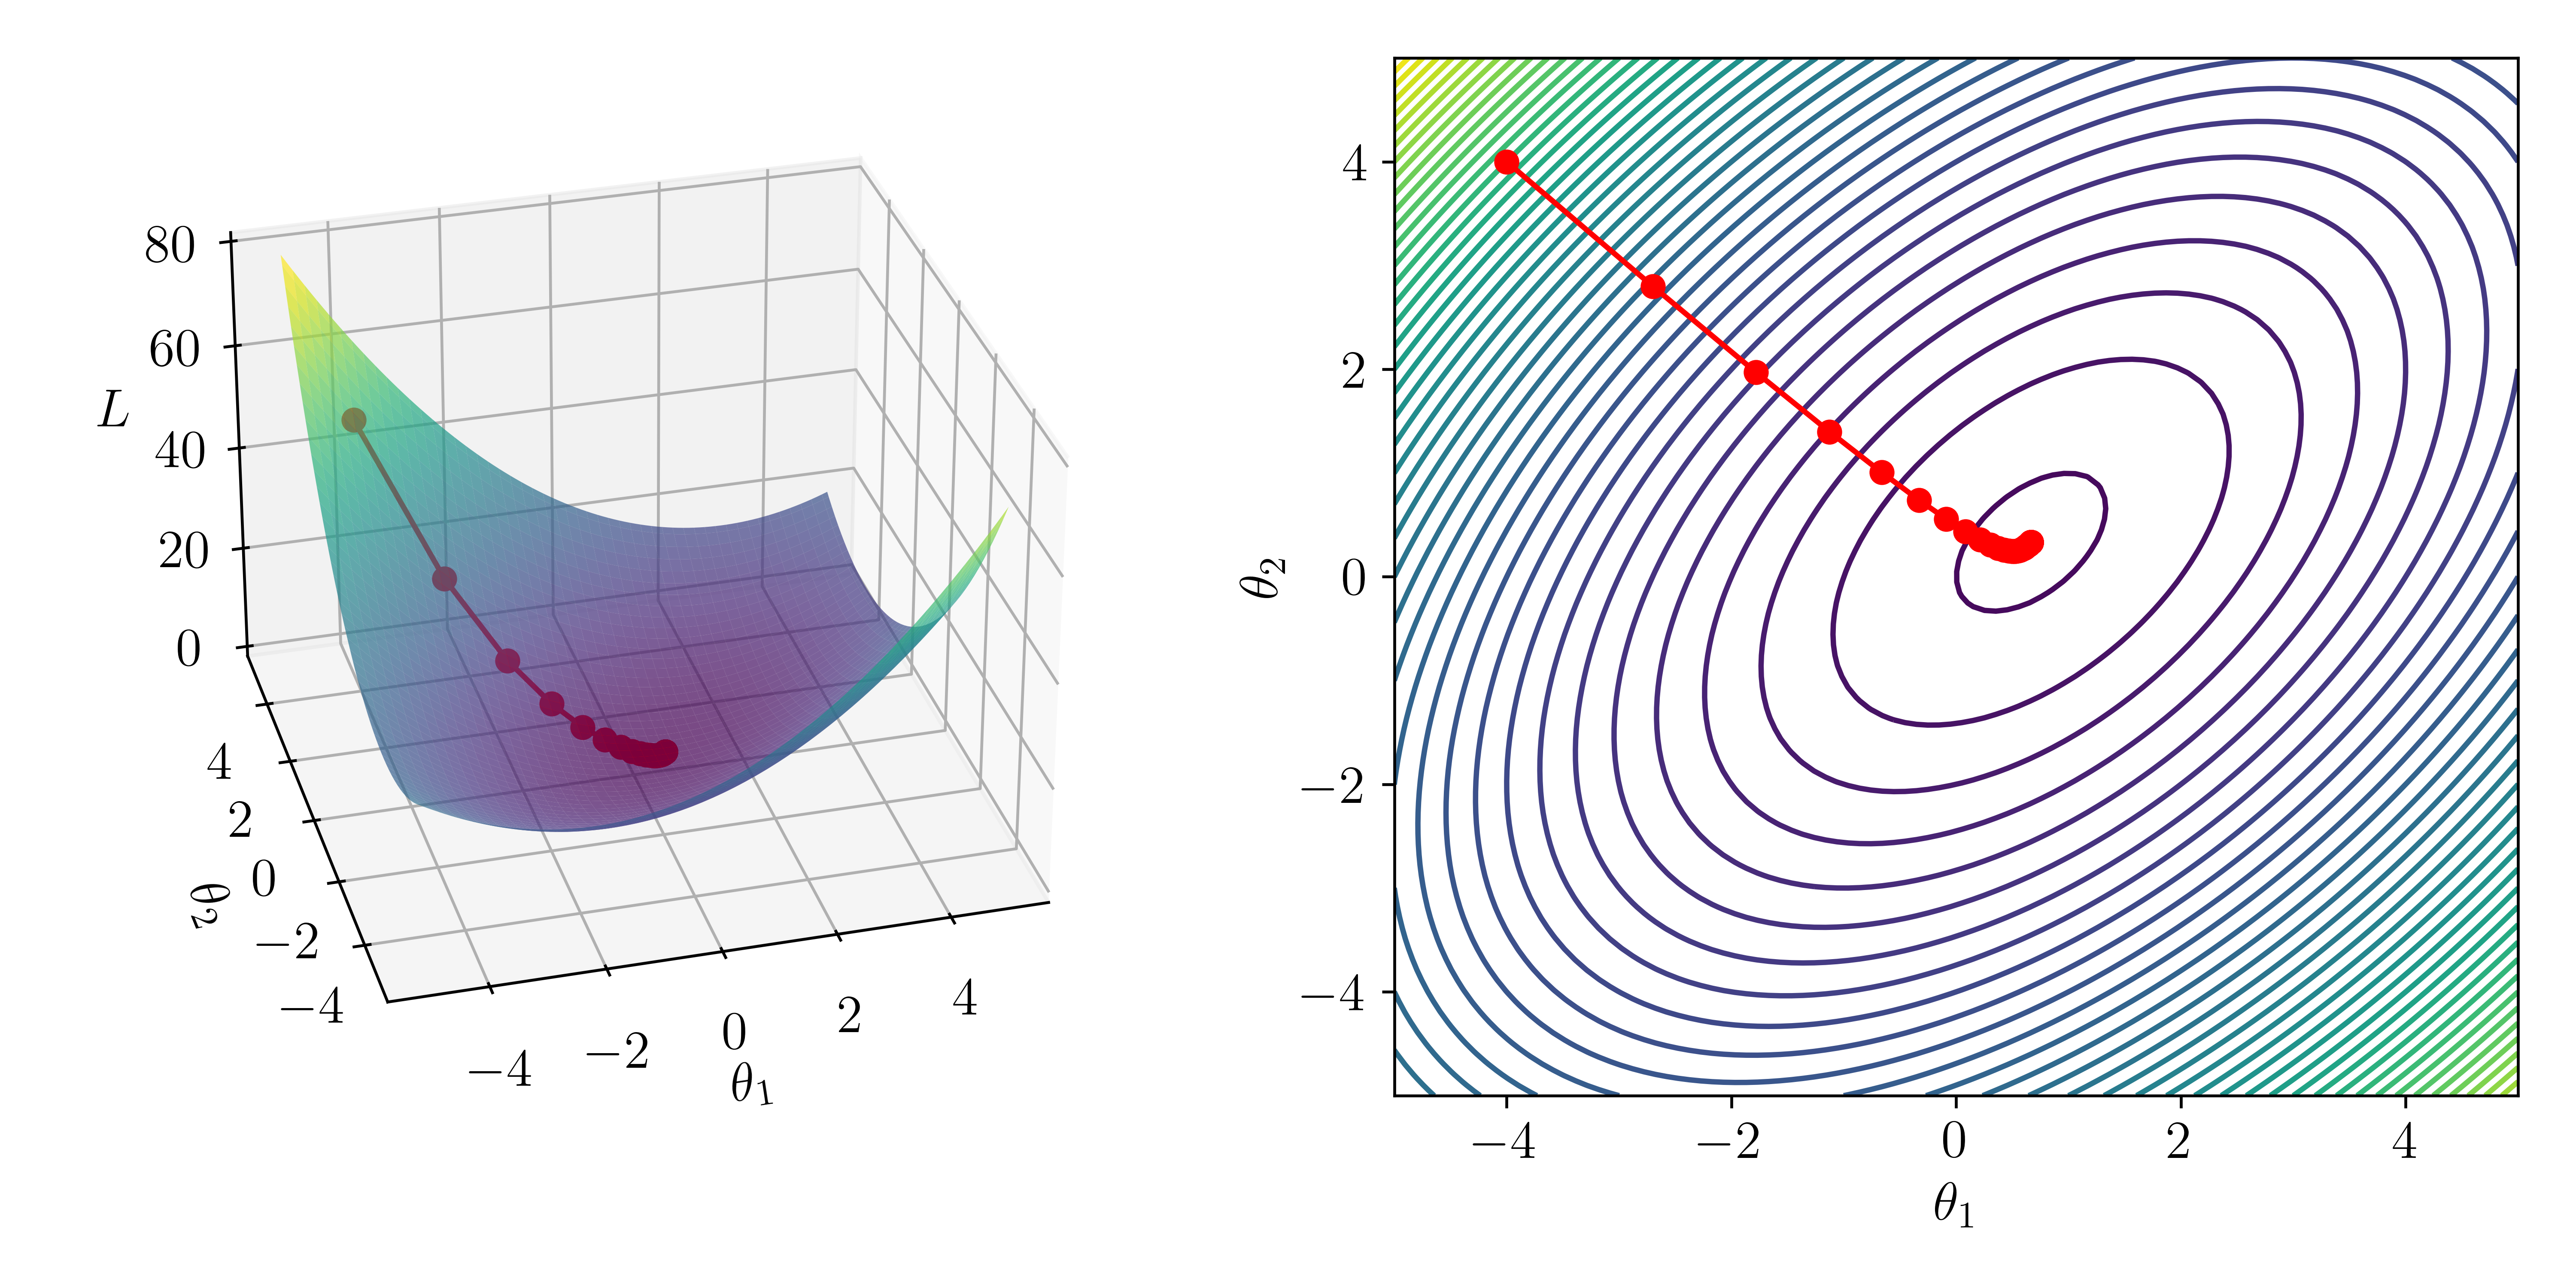
\includegraphics[width=\linewidth]{figs/gradient_descent.png}
    \caption{Visualization of naive gradient descent on the Himmelblau function \cite{jamil_literature_2013} by a 3D plot (left), and a contour plot (right). The red line shows $100$ iterations of gradient descent, starting from intial parameters $\boldsymbol{\theta}^{(0)} = [1,7]$, with $\eta = 0.001$. Local minima are marked with $\times$. (Original)}
    \label{fig:enter-label}
\end{figure}

In practice, some conditions may be defined to determine when to cease training, such as setting an upper limit on the number of iterations, setting a time limit, or setting a threshold for a satisfactory value of $L$. These values that modify aspects of a model's learning are called \textbf{\glspl{hyperparameter}}. Hyperparameter optimization is itself a complex topic that is beyond the scope of this section.

When $\boldsymbol{\theta}$ reaches a critical point ($\nabla L = 0$), the updates to $\boldsymbol{\theta}$ vanish, and the algorithm has reached a stable ending point. In an ideal case, this would be the global minima of $L$, the best that the model could possibly reach given the training data. In reality, reaching the global minima is highly improbable, $\boldsymbol{\theta}$ is much more likely to be stuck at a local minima, or a saddle point. We will discuss methods to overcome these challenges in Section~\ref{sec:gradient-descent-methods}.

\section{Neural Networks (NNs)}\label{sec:nn}

\textbf{\Glspl{ann}} often shortened to \textbf{\glspl{nn}}, are one of the largest classes of models used in machine learning. NNs are composed of \textbf{\glspl{node}} that are arranged in layers. The first layer is called the \textbf{input layer}, and the last layer is called the \textbf{output layer}. All layers in between are called \textbf{hidden layers}. NNs are usually fully connected, meaning that each node in a layer is considered by every node in the next layer.

\begin{figure}[h]
    \centering
    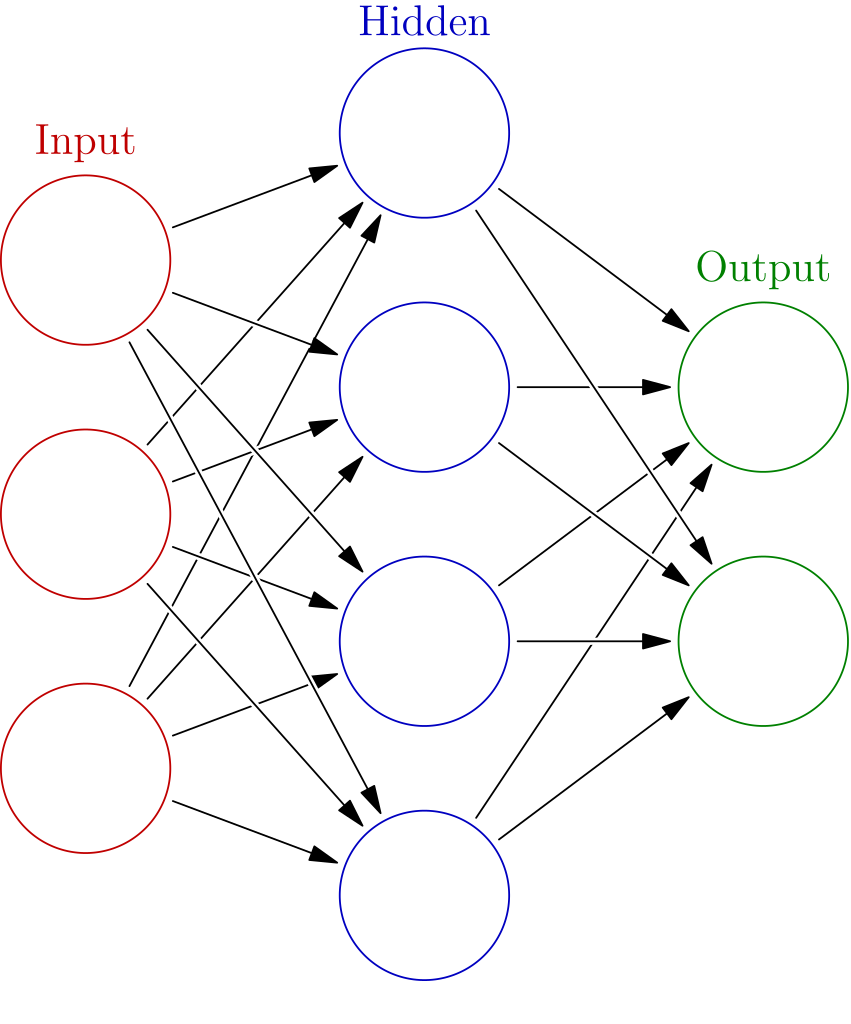
\includegraphics[width=0.3\linewidth]{figs/colored_neural_network.png}
    \caption{A schematic of a neural network with a input layer with three nodes, one hidden layer with four nodes, and an output layer with two nodes~\cite{commons_filecolored_2025}.}
    \label{fig:enter-label}
\end{figure}

Each node takes a biased weighted sum of the values of the previous layer, applies an activation function $\phi$, and outputs the value to the next layer.
\begin{equation} \label{eq:node}
    a^{(l)}_j = \phi\left(b_j^{(l)} + \sum_i w_{ij}^{(l)} a_i^{(l-1)}\right)
\end{equation}
Or, using matrix notation, where we define $\phi$ to act component-wise on a vector,
\begin{equation}
    \mathbf{a}^{(l)} = \phi\left(\mathbf{b}^{(l)} + \mathbf{W}^{(l)}\mathbf{a}^{(l-1)}\right).
\end{equation}
$\phi$ is usually the same for every layer of a netowrk, but it may not always be, in which case it may be specified with a subscript, $\phi^{(l)}$. The notable case where this arises is the softmax function for the final layer of a classification network. See Section~\ref{sec:classification} for more details.

In this article, we will use the notation $a^{(l)}_i$ to refer to the output of node $i$ in layer $l$, and $\mathbf{a}^{(l)}$ to refer to the vector of outputs of all nodes in layer $l$. The weights and biases applied onto nodes from layer $l-1$ to be inputted into the activation function of layer $l$ will be denoted as $\mathbf{W}^{(l)}$ and $\mathbf{b}^{(l)}$, respectively. In general, supercripts will denote a layer in the network, and subscripts will denote a specific component of a vector or matrix, such as a specific node or weight of a layer, as described in Section~\ref{notation}. Note that this superscript notation is different from the one we use with $\boldsymbol{\theta}^{(t)}$, which is used to denote the iteration of the gradient descent algorithm.

\subsection{Activation Functions}

For virtually all non-trivial problems, linear relationships are far too reductive to completely capture the complexity of the task at hand. Therefore, a variety of non-linear \textbf{activation functions} are applied at each node to eliminate this kind of model bias to allow the model to learn more non-linear relationships.

\textbf{Sigmoid functions} are ubiquitous in this role, and they are also useful since they normalize the output of a node to be between $0$ and $1$. This is useful for many applications, such as when the output of a node is interpreted as a probability.
\begin{equation}
    \sigma(x) = \frac{1}{1+e^{-x}}
\end{equation}
Another very common activation function is the \textbf{\gls{relu}}, which has the advantage of being computationally easier to calculate.
\begin{equation}
    \text{ReLU}(x) = \max(0,x)
\end{equation}
\begin{figure}[h]
    \centering
    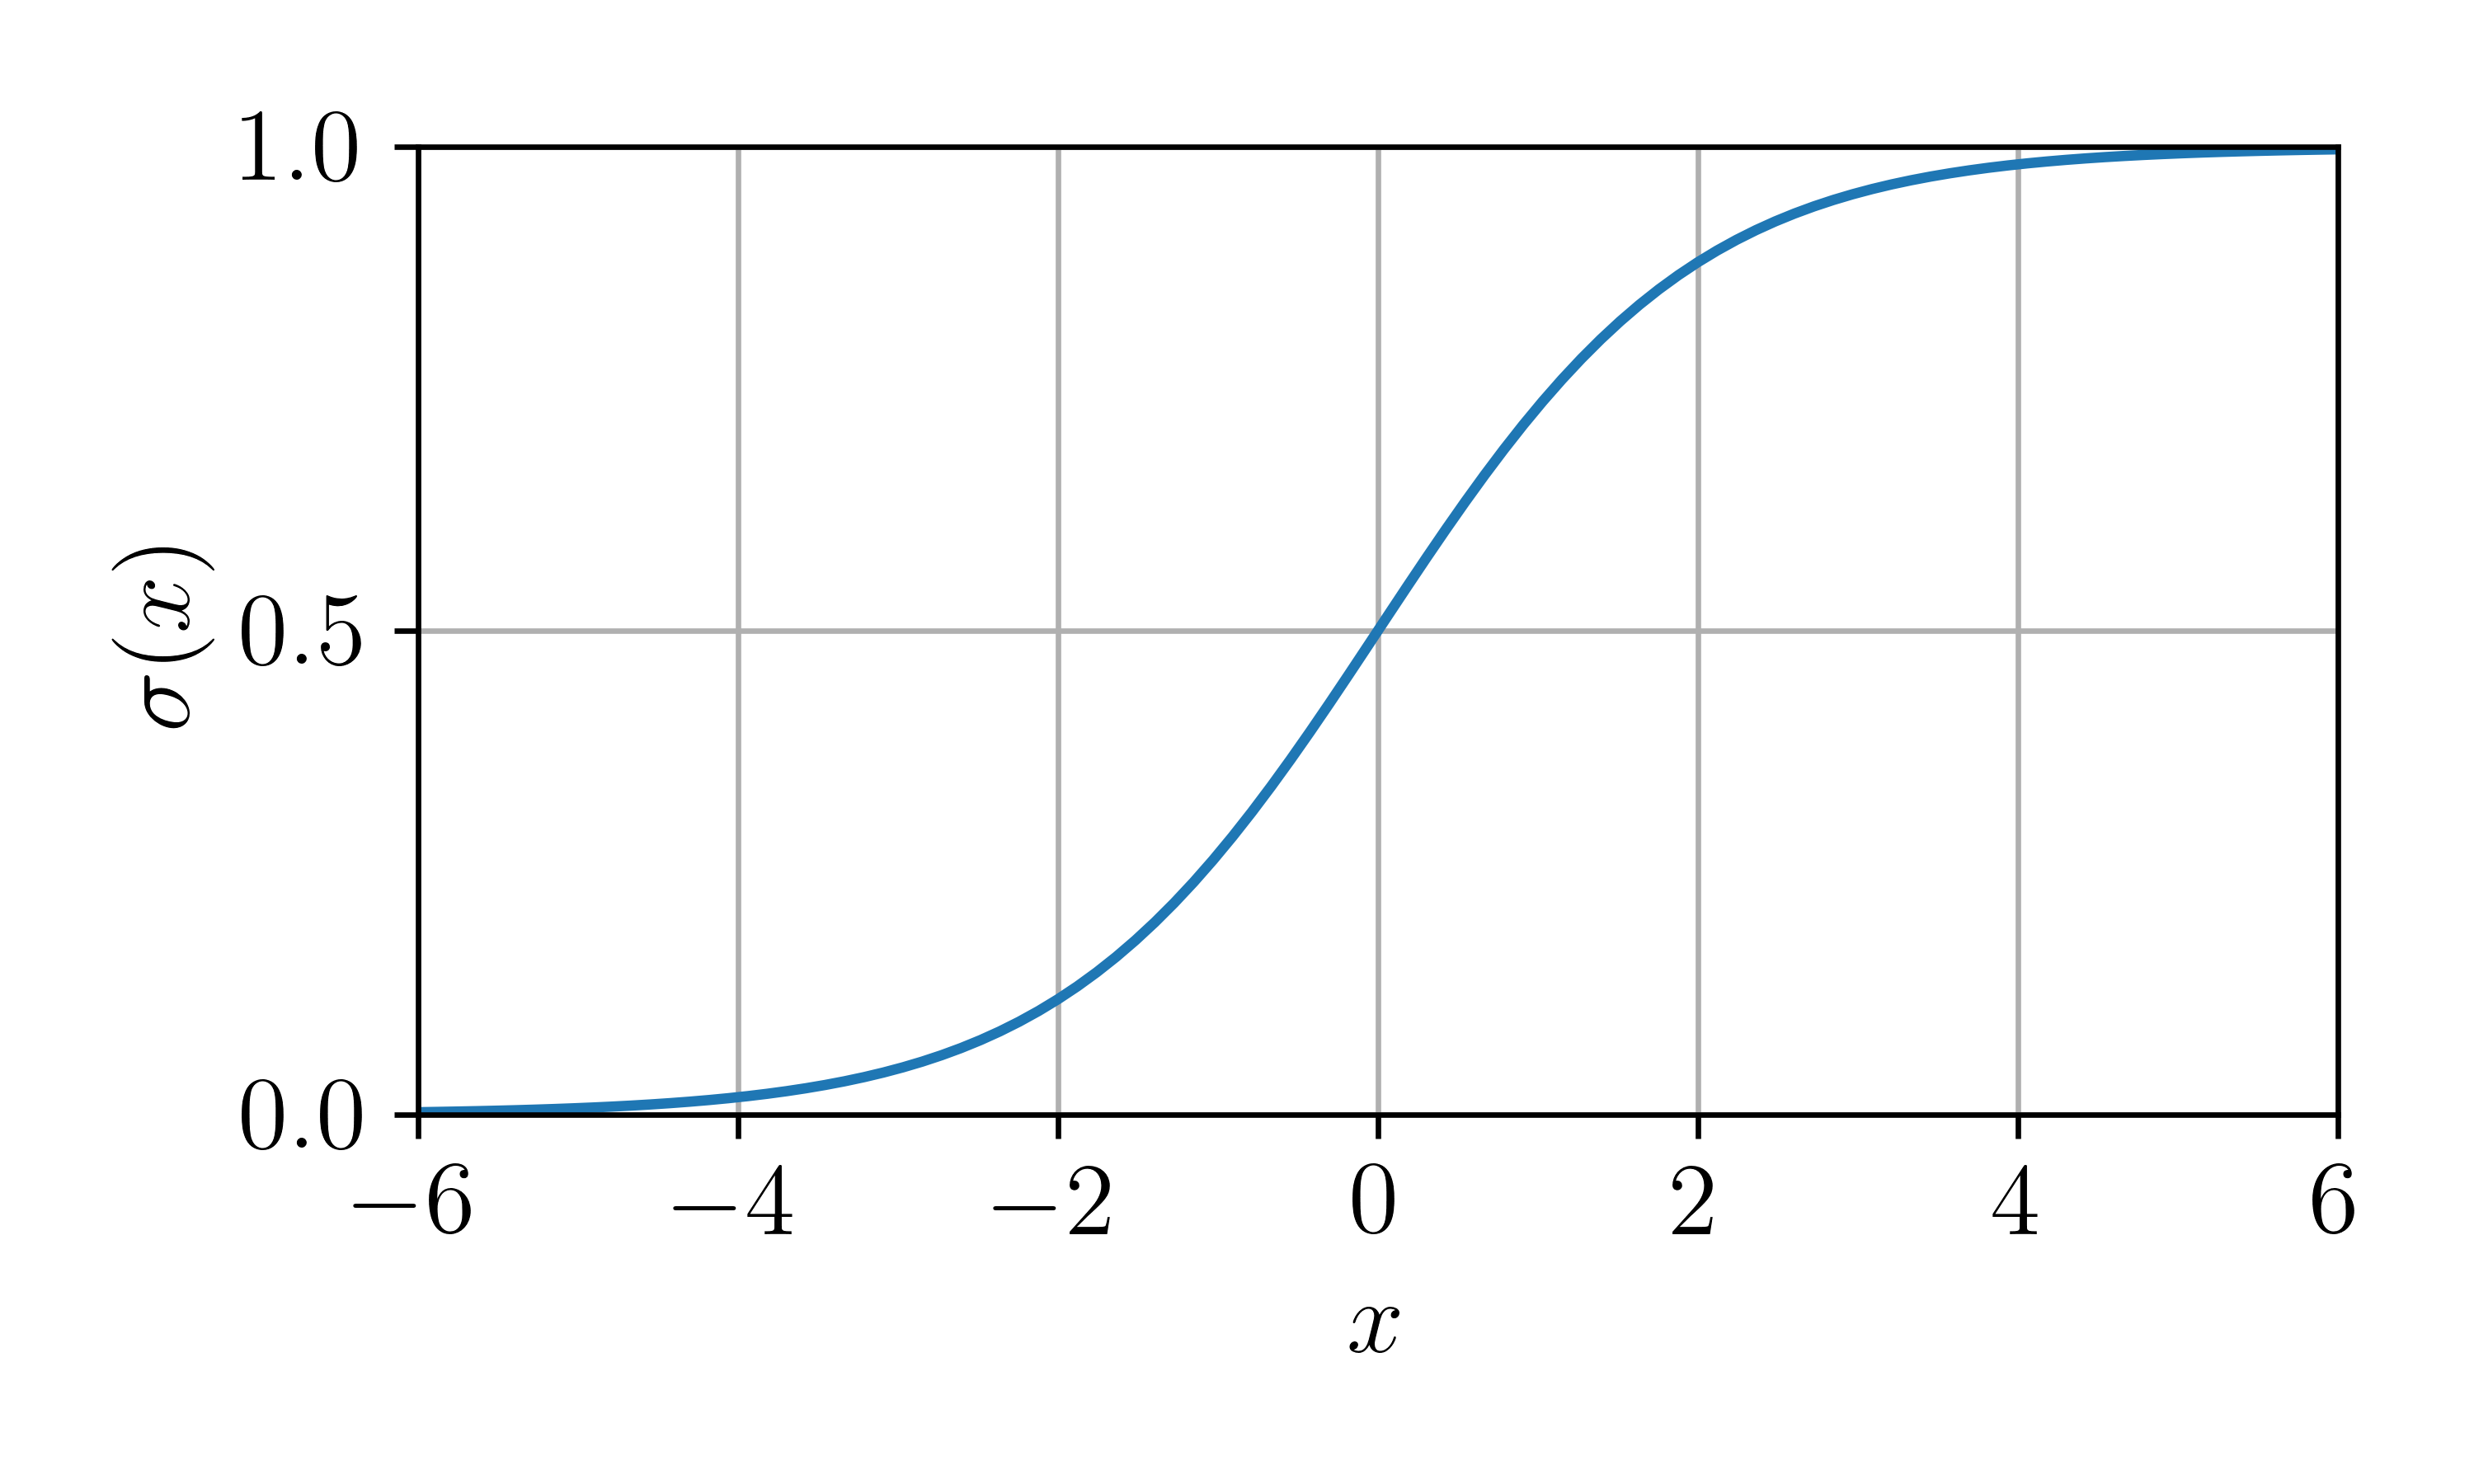
\includegraphics[width=0.45\linewidth]{figs/sigmoid.png}
    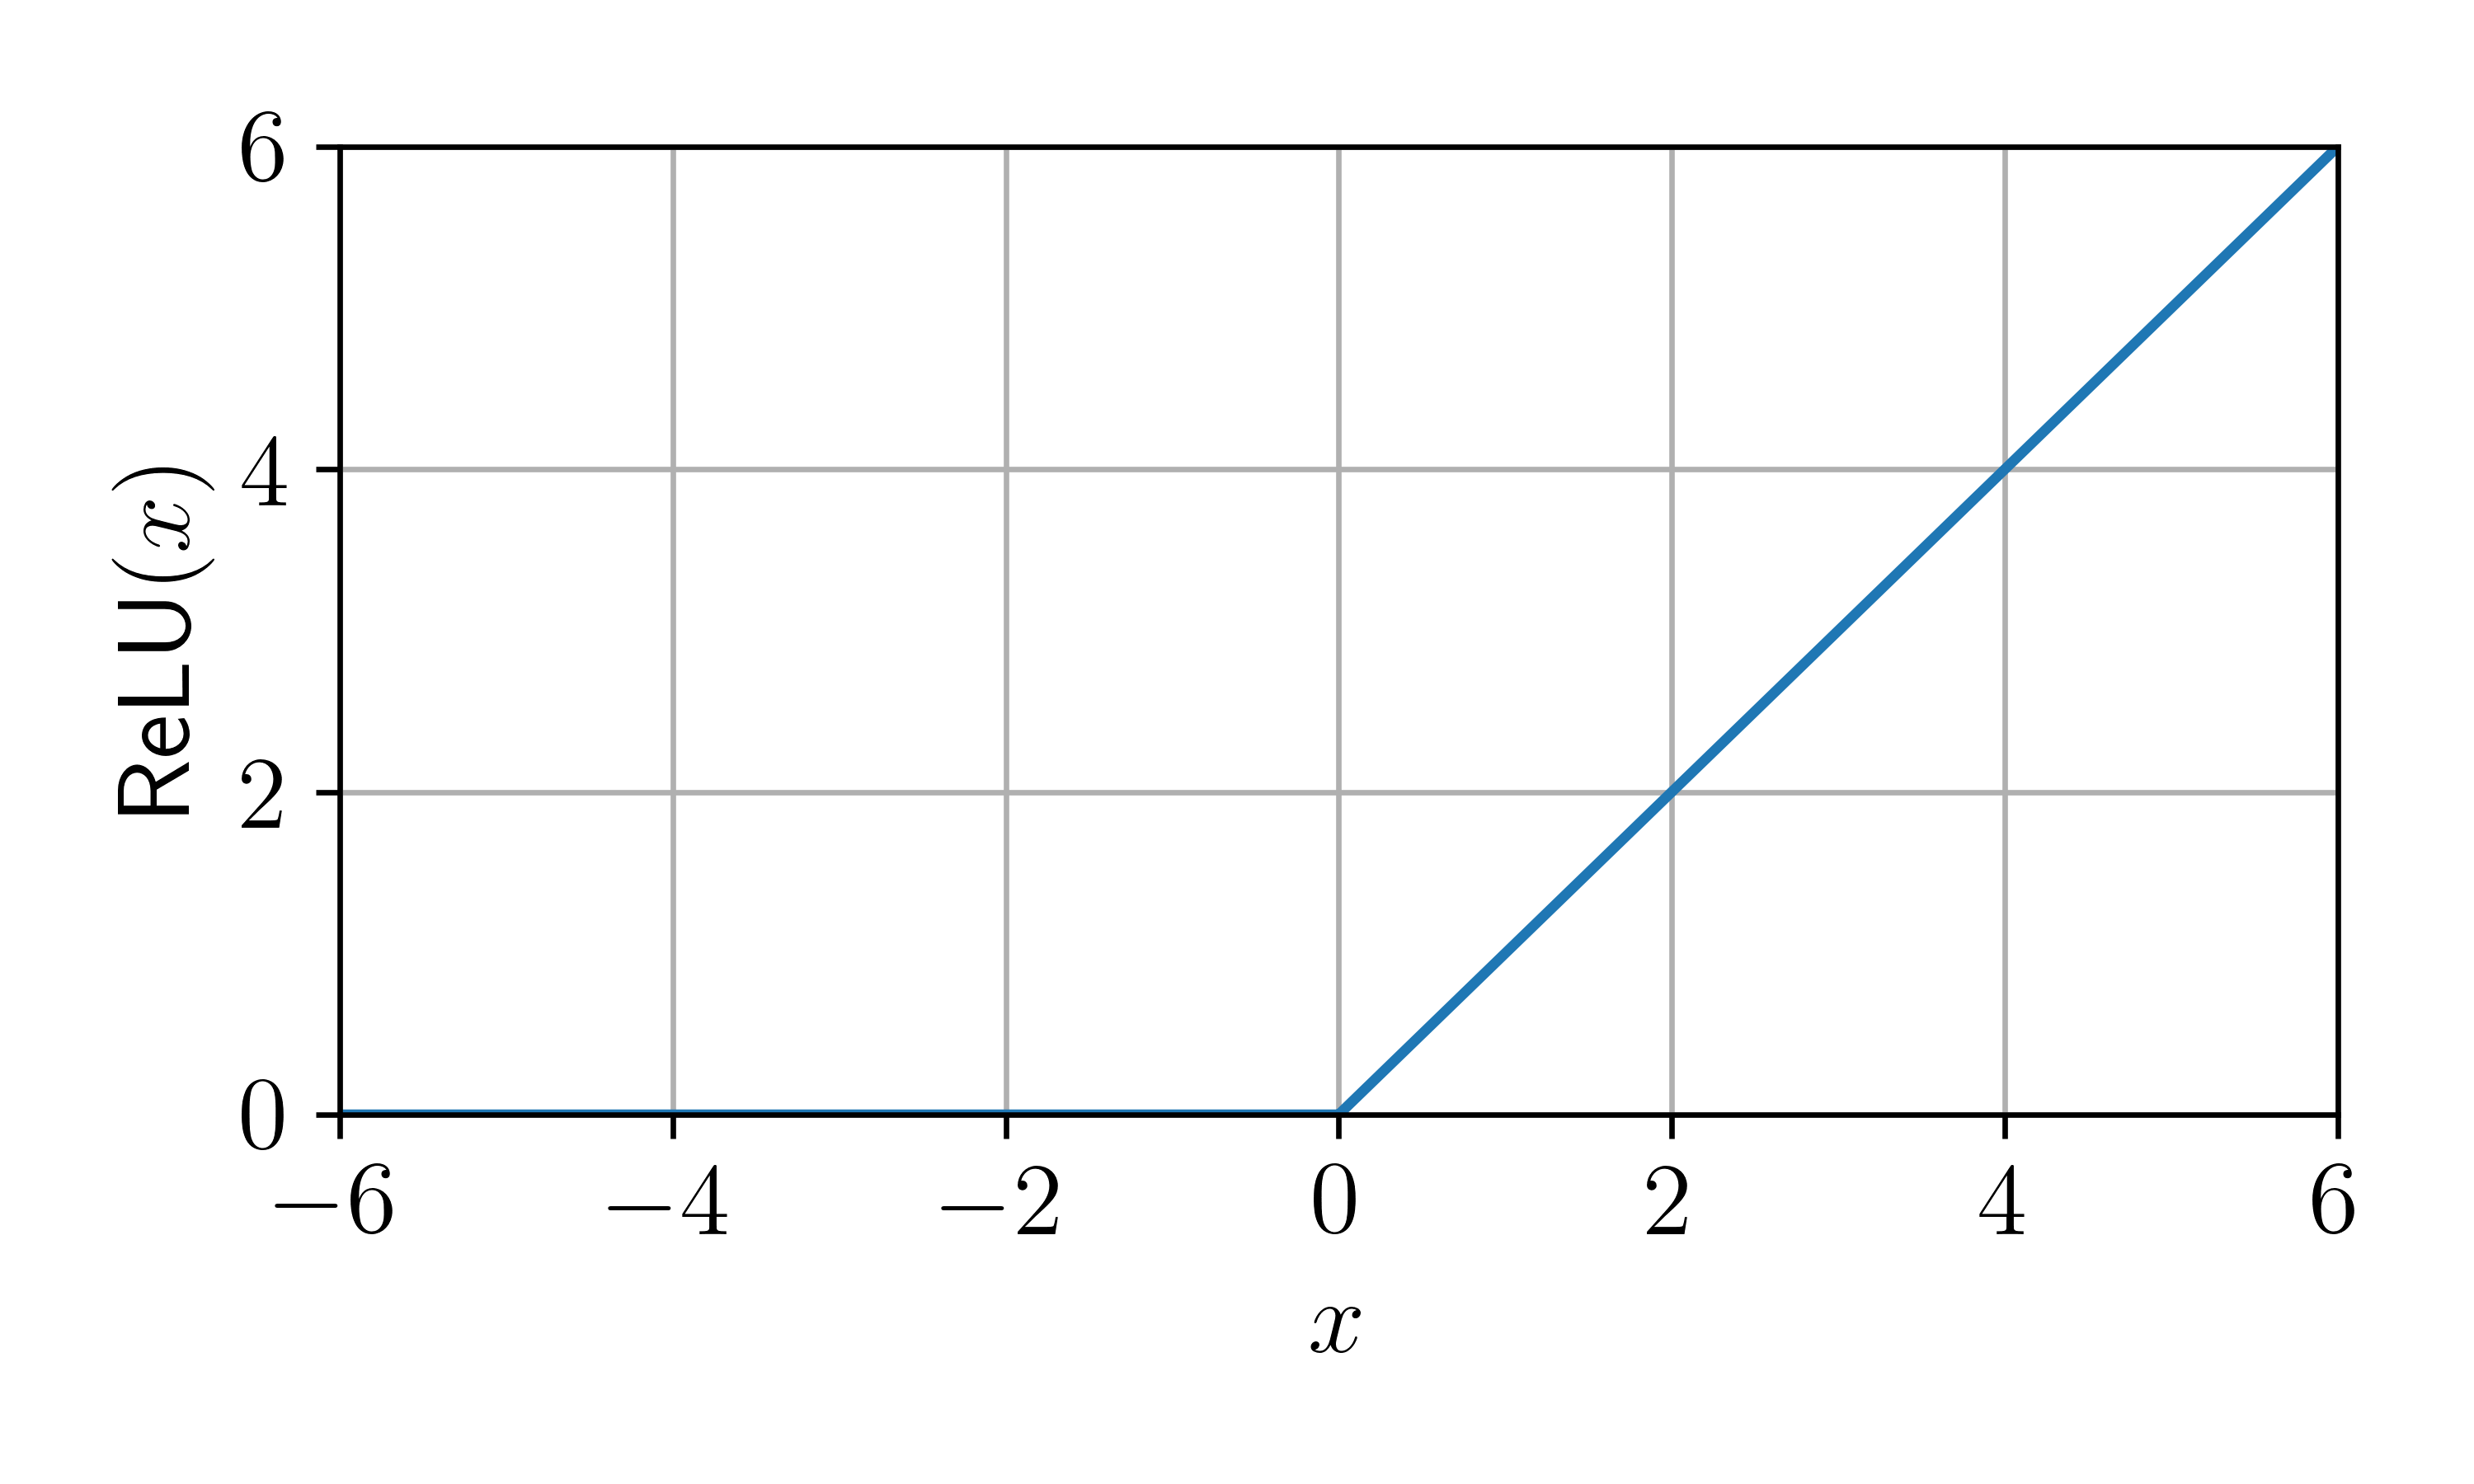
\includegraphics[width=0.45\linewidth]{figs/relu.png}
    \caption{Plot of $\sigma(x)$ (left) and $\text{ReLU}(x)$ (right). (Original)}
    \label{fig:enter-label}
\end{figure}

Any continuous relationship between two variables can be approximated by a \textit{sufficiently large} linear combination of sigmoid functions~\cite{cybenko_approximation_1989}.
\begin{equation} \label{eq:approximation}
    f \approx b + \mathbf{c} \cdot \sigma(\mathbf{b} + \mathbf{W}\mathbf{x}).
\end{equation}
Equation \ref{eq:approximation} is equivalent to a neural network with one hidden layer and scalar output (omitting the final application of an activation function).
\begin{figure}[h]
    \centering
    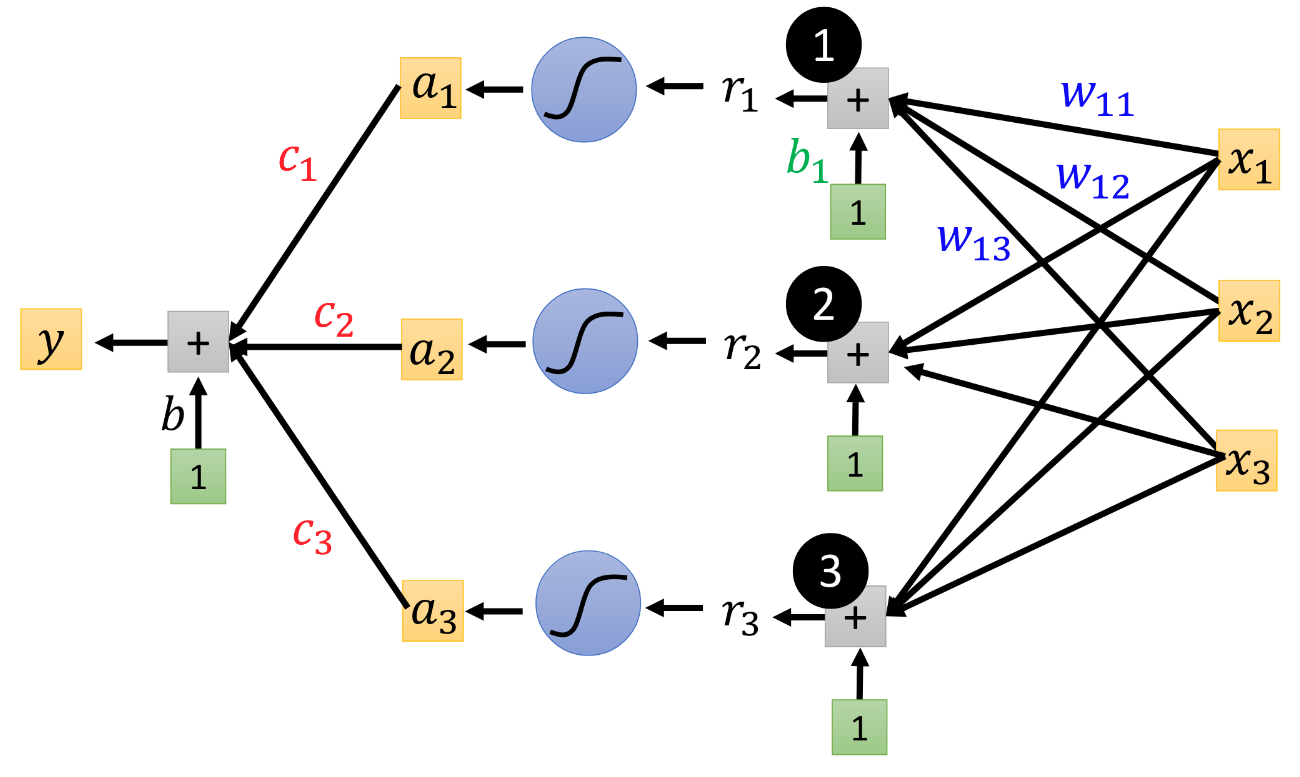
\includegraphics[width=0.5\linewidth]{figs/simple.png}
    \caption{Reprinted from \cite{lee_introduction_2021}.}
    \label{fig:enter-label}
\end{figure}

This result can be generalized to any non-polynomial activation function, including ReLUs, in the \textbf{universal approximation theorems}, implying that neural networks that use such activation functions may theoretically learn any relationship given \textit{sufficiently large} amounts nodes and layers~\cite{hornik_multilayer_1989, kidger_universal_2020, pinkus_approximation_1999}. This property of neural networks become especially useful in other areas of machine learning where aribtrary function approximators are needed. Though, it is important to note that this result is only theoretical, and in practice, computational and data constraints usually frustrate this ideal.

\subsection{Layers}

The addition of layers to a model increases its complexity, the number of which is referred to as its \textbf{depth}. The number of nodes in a layer is referred to as the layer's \textbf{width}. The width and depth of a model are hyperparameters, and there is a balance to be made between model bias, computational demands, and overfitting, a phenomenon we will discuss in Section~\ref{sec:overfitting}.

The output layer of a model is tailored to the task at hand. A \textbf{regression} model predicts a single, continuous value, represented by a single node in the output layer, or a vector of continuous values, represented by multiple nodes in the output layer. In contrast, a \textbf{classification} model sorts inputs into discrete categories, usually with the final output layer being a vector of nodes, each representing a class, with the value of each node representing the probability that the input belongs to that class. The specific differences between these two types of models will be discussed in Section~\ref{sec:classification}.

\section{Backpropagation}

\textbf{Backpropagation} is the textbook algorithm for computing the gradient of the loss function. Essentially, it is the application of the chain rule to neural networks~\cite{nielsen_neural_2019,sanderson_backpropagation_2017}.

Recall Equation~\ref{eq:node},
\begin{equation}
    a^{(l)}_j = \phi^{(l)}\left(b_j^{(l)} + \sum_i w_{ij}^{(l)} a_i^{(l-1)}\right).
\end{equation}
For easier comprehension, define $z^{(l)}_j$ to be the weighted and biased sum of the previous layer that is the input to the activation function.
\begin{equation}\label{eq:weighted-sum}
    z^{(l)}_j = b_j^{(l)} + \sum_i w_{ij}^{(l)} a_i^{(l-1)}
\end{equation}
Then, we can rewrite the equation as
\begin{equation}\label{eq:simplified-node}
    a^{(l)}_j = \phi^{(l)}(z_j^{(l)}).
\end{equation}
Assuming a MSE loss, the loss for a single label is the squared difference each node of the output layer $a^{(L)}_j$ and the label $y_j$.
\begin{equation}
    C = \sum_j {(a^{(L)}_j - y_j)}^2
\end{equation}
In this section, we use $L$ to denote the output layer of the network, so we instead use the other standard $C$ to denote the loss function to avoid cconfusion.

We wish to compute the gradient of the loss by computing the partial derivative of the loss with respect to each parameter of the network. First, consider the weights and biases of the output layer, $w_{ij}^{(L)}$ and $b_j^{(L)}$. By the chain rule,
\begin{equation}\label{eq:chain-rule-weights}
    \frac{\partial C}{\partial w_{ij}^{(L)}} = \frac{\partial C}{\partial a_j^{(L)}} \frac{\partial a_j^{(L)}}{\partial z_j^{(L)}} \frac{\partial z_j^{(L)}}{\partial w_{ij}^{(L)}},
\end{equation}
and
\begin{equation}\label{eq:chain-rule-biases}
    \frac{\partial C}{\partial b_j^{(L)}} = \frac{\partial C}{\partial a_j^{(L)}} \frac{\partial a_j^{(L)}}{\partial z_j^{(L)}} \frac{\partial z_j^{(L)}}{\partial b_j^{(L)}}.
\end{equation}

For paramaters in the previous layers, we can simply apply the chain rule recursively.
\begin{equation}\label{eq:big-chain}
    \frac{\partial C}{\partial a_j^{(L)}} \underbrace{\frac{\partial a_j^{(L)}}{\partial z_j^{(L)}} \frac{\partial z_j^{(L)}}{\partial a_j^{(L-1)}}}_{\text{output layer $L$}} \underbrace{\frac{\partial a_j^{(L-1)}}{\partial z_j^{(L-1)}} \frac{\partial z_j^{(L-1)}}{\partial a_{j}^{(L-2)}}}_{\text{layer $L-1$}} \cdots \underbrace{\frac{\partial a_j^{(l)}}{\partial z_j^{(l)}} \left(\frac{\partial z_j^{(l)}}{\partial w_{ij}^{(l)}} \ \text{or} \ \frac{\partial z_j^{(l)}}{\partial b_j^{(l)}}\right)}_{\text{layer $l$}}
\end{equation}
Note the following:
\begin{equation}\label{eq:partial-z-partial-a}
    \frac{\partial a_j^{(L)}}{\partial z_j^{(L)}} = \phi^{(L)\prime}(z_j^{(L)}),
\end{equation}
\begin{equation}
    \frac{\partial z_j^{(l)}}{\partial a_{j}^{(l-1)}} = \sum_j w_{ij}^{(l)},
\end{equation}
\begin{equation}
    \frac{\partial z_j^{(L)}}{\partial w_{ij}^{(L)}} = a_i^{(L-1)},
\end{equation}
\begin{equation}
    \frac{\partial z_j^{(L)}}{\partial b_j^{(L)}} = 1.
\end{equation}
Substituting,

This notation is somewhat cumbersome, so we will introduce the standard notation used found in literature. Let $\nabla_{a^{(L)}}C$ be the vector of partial derivatives of the loss with respect to the output of the final layer $C$,
\begin{equation}
    \nabla_{a^{(L)}}C = \begin{bmatrix}
        \frac{\partial C}{\partial a_j^{(L)}} \\
    \end{bmatrix}.
\end{equation}
Next, define $\delta^{(l)}$ be the vector of partial derivatives of the loss with respect to the weighted and biased sum of the previous layer $z^{(l)}$,
\begin{equation}
    \delta^{(l)} = \begin{bmatrix}
        \frac{\partial C}{\partial z_1^{(l)}} \\
        \vdots
    \end{bmatrix}.
\end{equation}


Thus, we can recursively define $\delta^{(l)}$ by the following two equations:
\begin{equation}
    \delta^{(L)} = \nabla_{a^{(L)}}C \odot \phi'(z^{(L)}),
\end{equation}
\begin{equation}
    \delta^{(L-1)} = {\left(\mathbf{W}^{(L)}\right)}^T \delta^{(L)} \odot \phi'(z^{(L-1)}).
\end{equation}

Using Equation~\ref{eq:weighted-sum} and Equation~\ref{eq:simplified-node}, we can compute these terms as follows:
\begin{equation}
    \frac{\partial C}{\partial a_j^{(L)}} = 2(a_j^{(L)} - y_j)
\end{equation}

Substituting these terms into the equations, we have
\begin{equation}
    \frac{\partial C}{\partial w_{ij}^{(L)}} = 2(a_j^{(L)} - y_j) \phi'(z_j^{(L)}) a_i^{(L-1)}.
\end{equation}

wow this is really complicated to explain with math will come back later

\section{Overfitting}\label{sec:overfitting}
\textbf{Overfitting} is a phenomenon that occurs when a model learns the training data too well, and is unable to generalize to new data. Generally, models with more parameters and degrees of freedom are more prone to overfitting. This may be mitigated by simply using a smaller model or by stopping training earlier, but these methods are not always feasible. Sometimes, there may be a fundamental difference between the training data and the test data that prevents any progress from being made. In general, we call problems of this nature \textbf{mismatches}, \textbf{distribution shifts}, or \textbf{dataset shifts}.

Models are usually tested on a seperate data set as a metric of how accurete their predictions are. An indicator of overfitting is when the model performs well on the training data, but poorly on the test data.

\begin{figure}
    \centering
    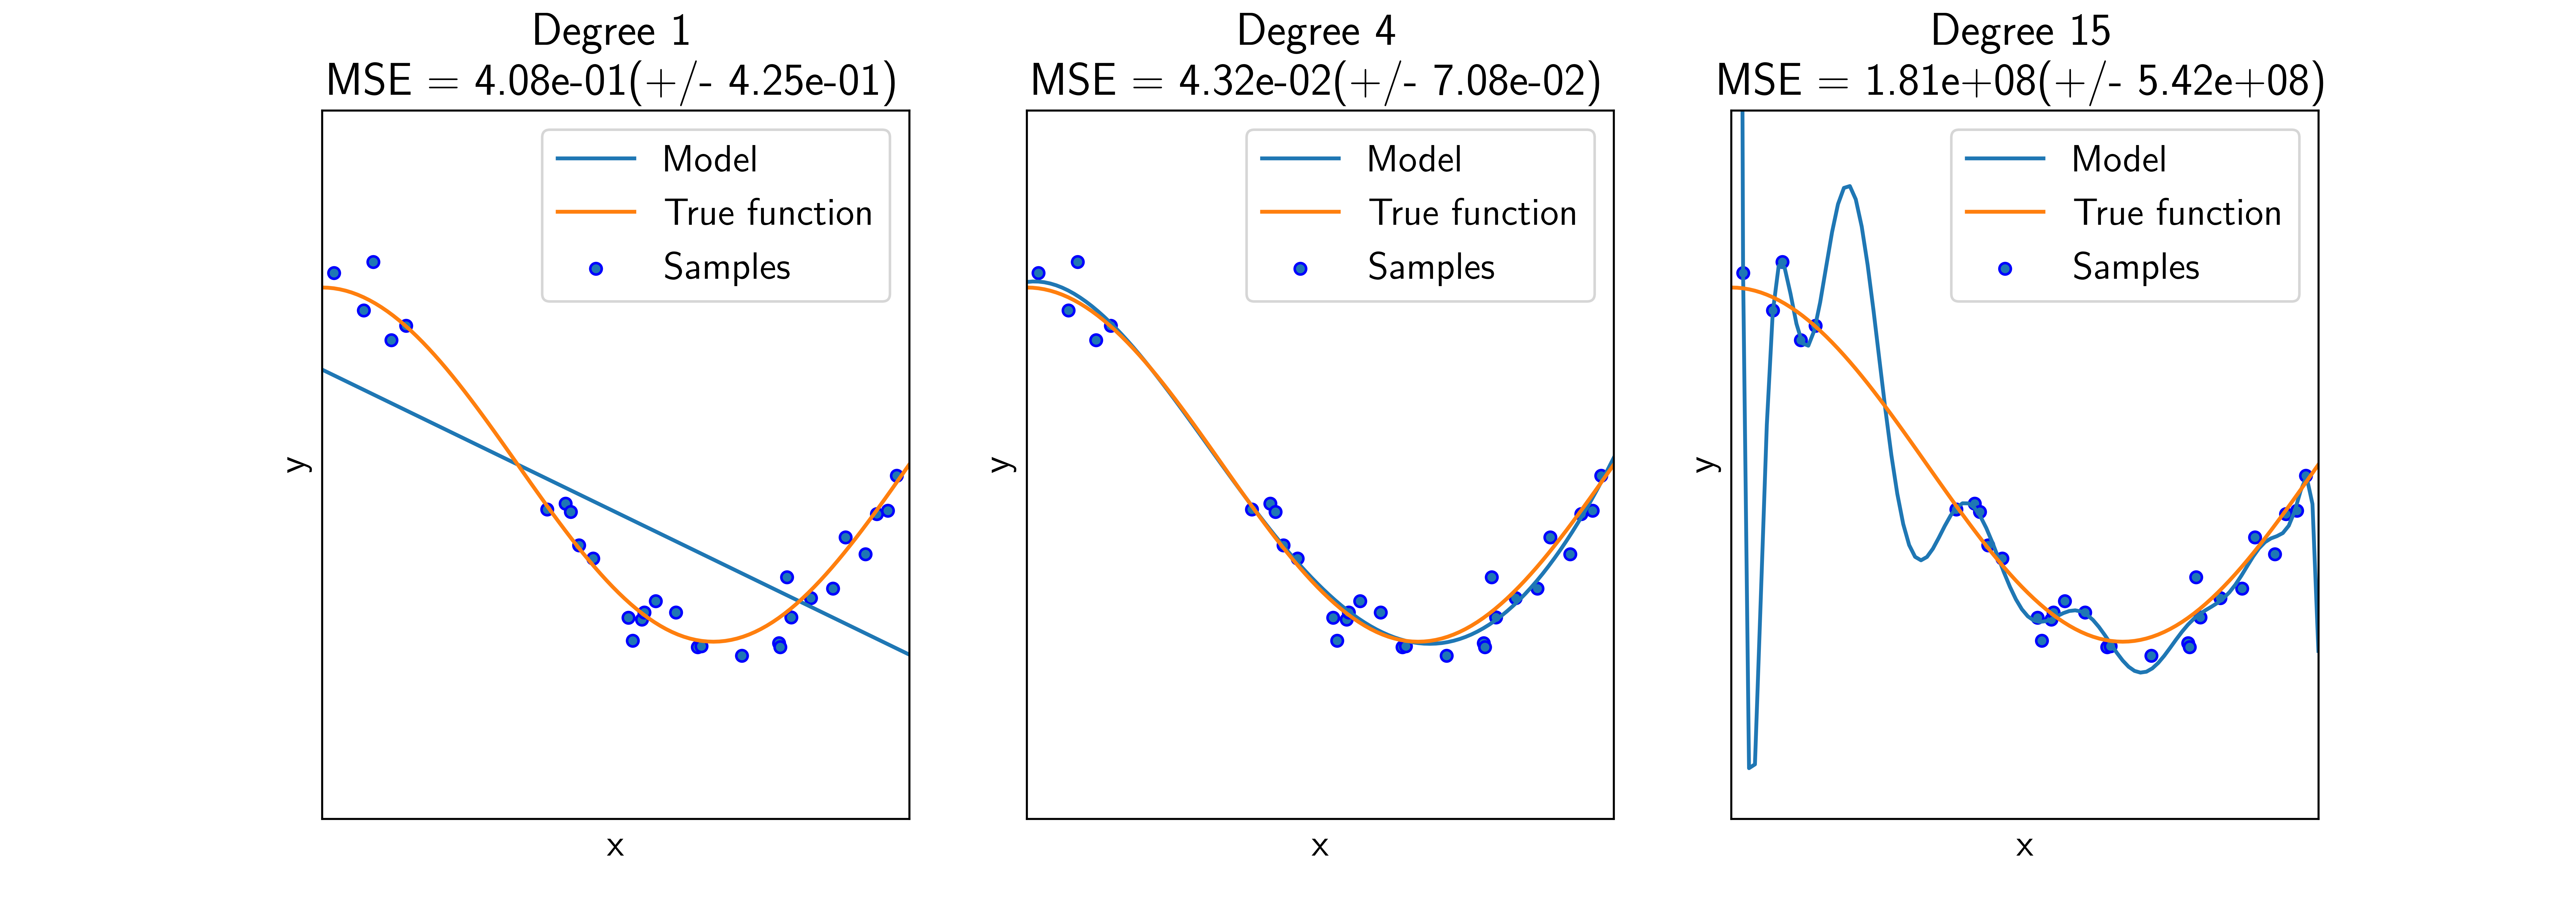
\includegraphics[width=\linewidth]{figs/underfitting_overfitting.png}
    \caption{Polynomial models of different degrees fitted to sample data. Modified from documentation for \texttt{scikit-learn}~\cite{pedregosa_scikit-learn_2011}.}
    \label{fig:overfitting}
\end{figure}

The degree $1$ polynomial in the left of Figure~\ref{fig:overfitting} is underfitted and has too much model bias, while the degree $15$ polynomial on the right is overfitted and has too much model variance.

\subsection{Cross-validation}
\textbf{Cross-validation} is a technique for estimating the performance of a model on unseen data, from only the training set. This ensures that any signs of overfitting can be monitored during training. Cross-validation splits the training data into a training set and a validation set. The model is trained on the training set, and the performance is evaluated on the validation set. This process is repeated for different partitions of the training data, and the average performance is taken as the final metric.

Cross-validation can be exhaustive where every possible partition is evaluated (leave-one-out cross-validation), though this is usually infeasible for large datasets.

\subsubsection{$k$-fold cross-validation}
The most common variant of cross-validation is $k$-fold cross-validation, a non-exhaustive method that randomly partitions the training data into $k$ equally sized subsets called \textbf{folds}.

\begin{figure}[h]
    \centering
    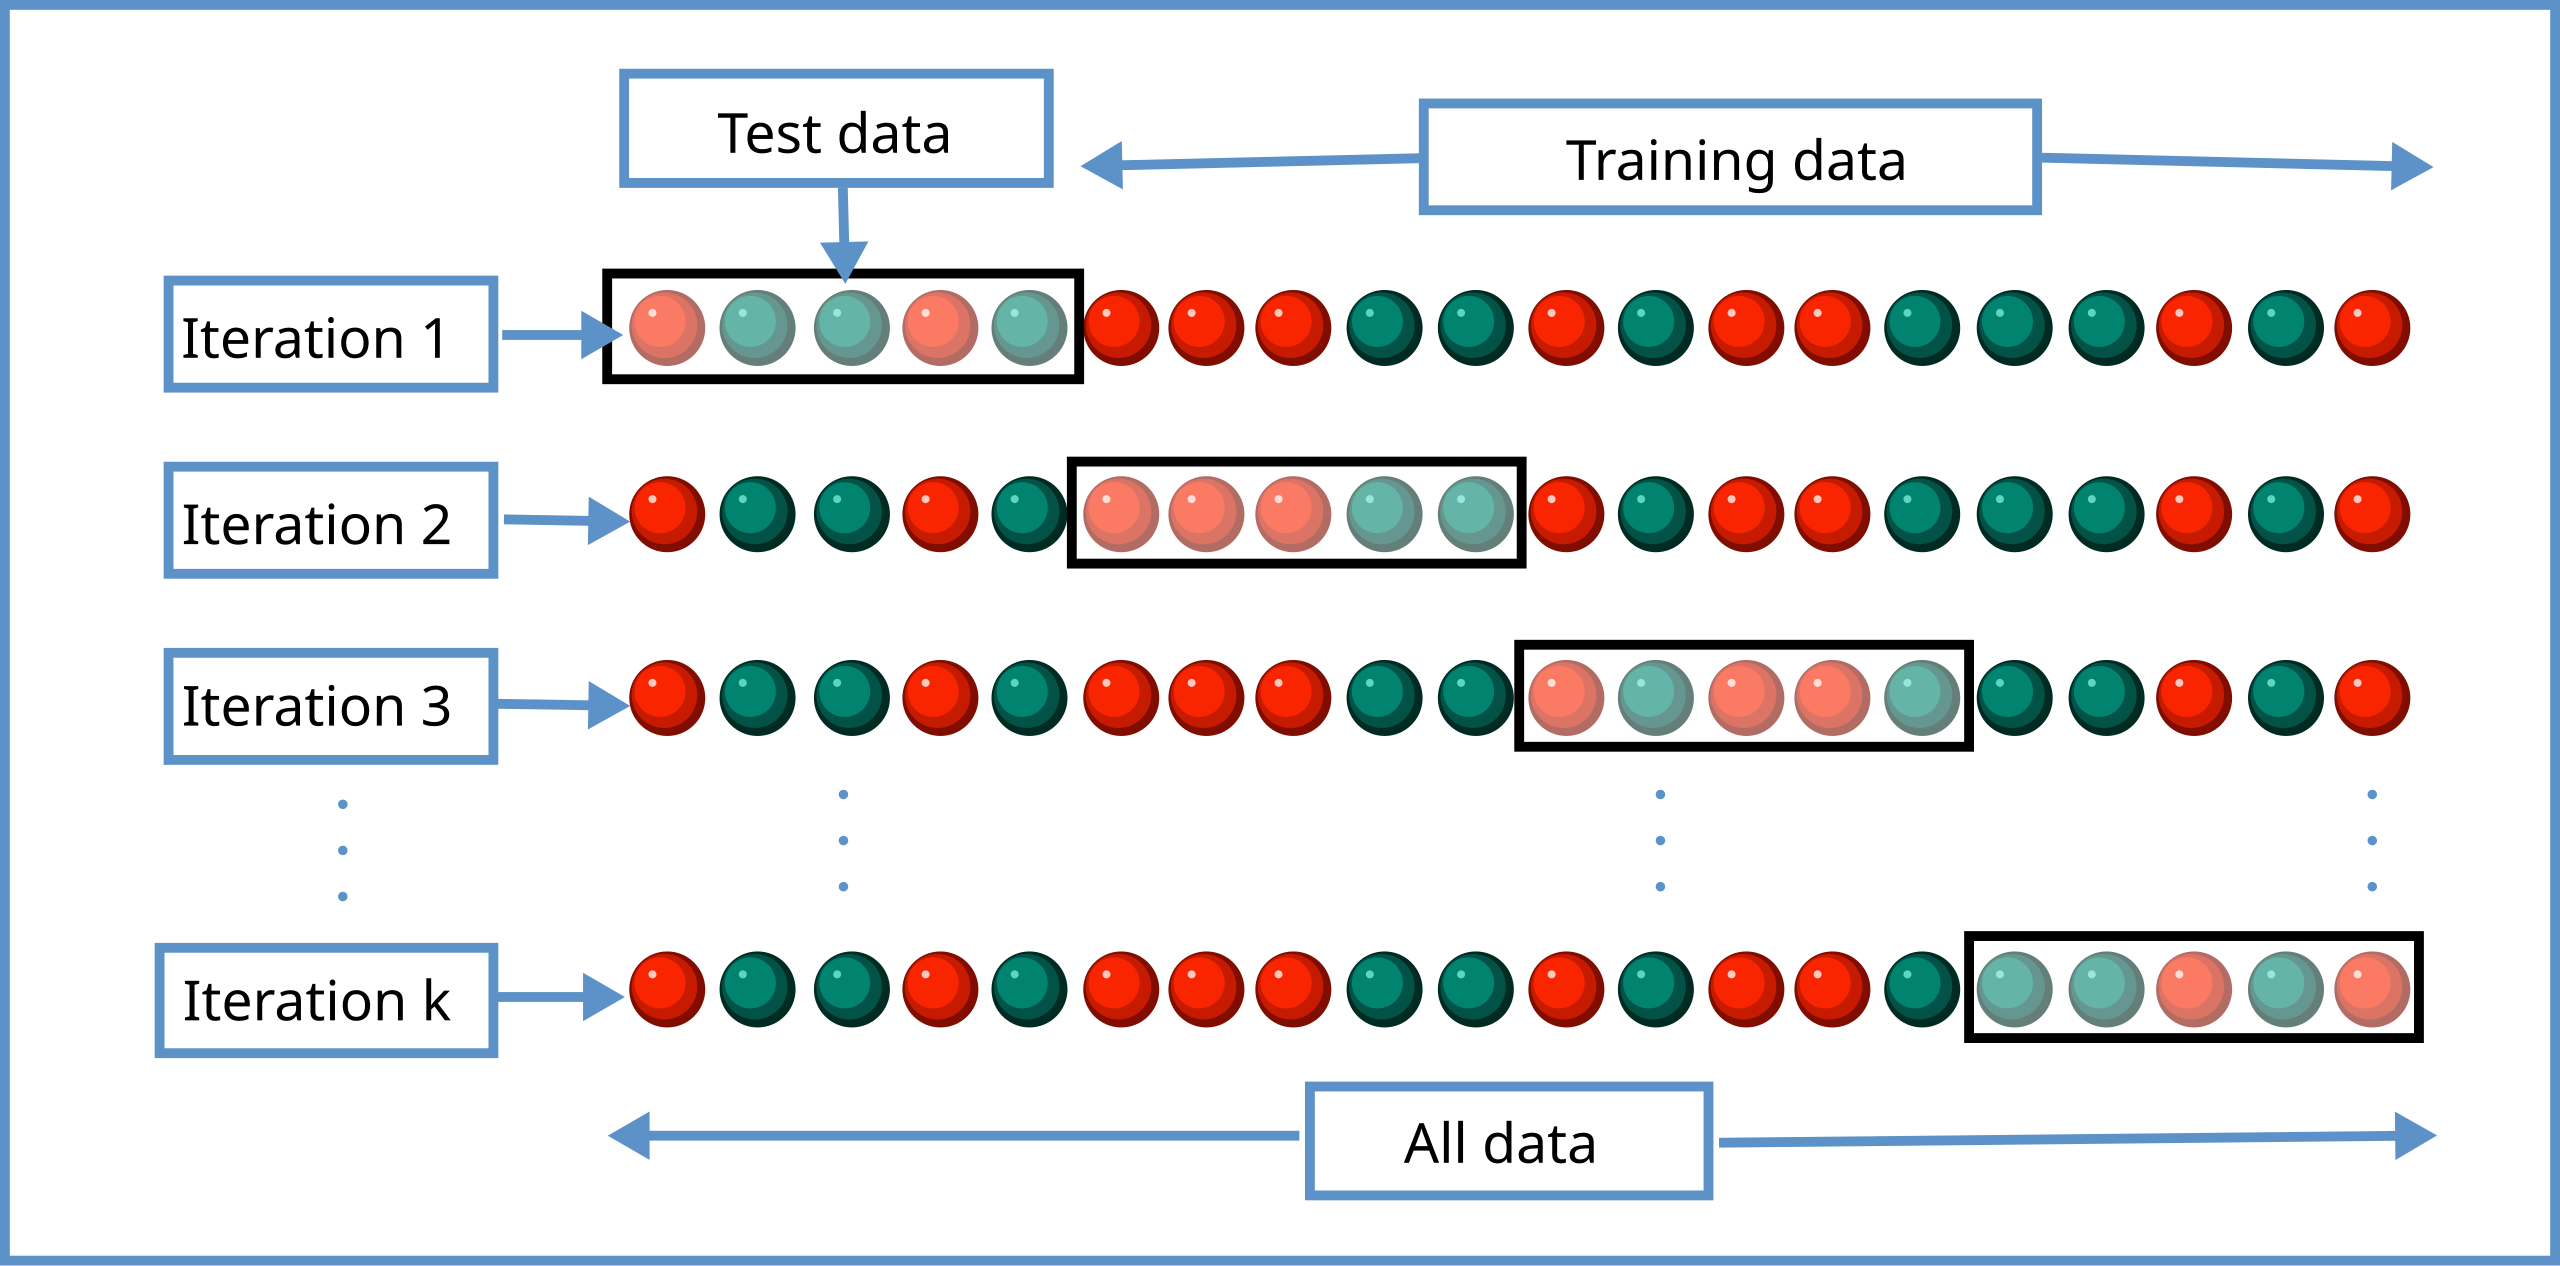
\includegraphics[width=\linewidth]{figs/kfold_cross_validation.png}
    \caption{\cite{commons_filek-fold_2024}}
    \label{fig:enter-label}
\end{figure}

$k$ is a hyperparameter, usually set to $5$ or $10$. The model is trained on $k-1$ folds, and the performance is evaluated on the remaining fold. This process is repeated for all combinations of folds, for a total of $k$ iterations. Essentially, this is leave-one out applied to blocks of data rather than individual data points. The performance is averaged over all $k$ iterations to give a final performance metric that is much more robust to overfitting than an unpartitioned training set

\subsection{Regularization}

learn more about this

\subsection{Dropout}
learn more about this


\section{Data Batching}

Rather than considering the entire training dataset all at once, we can iterate through small subsets of the training data, called \textbf{\glspl{batch}}, and compute gradient descent on that subset, updating parameters every batch. This is called \textbf{mini-batch gradient descent}, as opposed to \textbf{batch gradient descent}, which considers the entire training data set. (The author despises this inconsistent terminiology as much as you do.) After all batches have been iterated through, the model is said to have completed one \textbf{epoch} of training. The dataset is then shuffled, and the process is repeated for a specified number of epochs.

The size of a batch and the number of epochs to train for are both hyperparameters.

% ehh look into this more
Batching also has the advantage of being able to parallelize the computation of the gradient, as each batch can be computed independently. Thus, \textbf{graphics processing units} (GPUs) and \textbf{tensor processing units} (TPUs) are highly effective for training neural networks, with training times reduced by orders of magnitude with hardware acceleration.

\subsection{Batch size}

\subsection{Stochastic Gradient Descent}

Rather than computing the gradient of the loss function over the entire training data set, \textbf{stochastic gradient descent} (SGD) iterates on every single example. This is much faster than the former method, usually called \textbf{batch gradient descent}, but it is also much noisier. However, a noisy path may not necessarily be undesirable, as it may help the model escape local minima and saddle points.

\begin{algorithm}
    \caption{Stochastic gradient descent with learning rate $\eta$ over N epochs.}\label{alg:sgd}
    \begin{algorithmic}[1]
        \State Initialize parameters $\boldsymbol{\theta}$
        \For{$i = 1, \ldots, N$}
            \State Shuffle dataset
            \ForAll{example $\mathbf{x}$ in dataset}
                \State Compute gradient of loss $\nabla L_\mathbf{x}(\boldsymbol{\theta})$ with respect to $\mathbf{x}$
                \State $\boldsymbol{\theta} \leftarrow \boldsymbol{\theta} - \eta \nabla L_x(\boldsymbol{\theta})$
            \EndFor
        \EndFor \\
        \Return $\boldsymbol{\theta}$
    \end{algorithmic}
\end{algorithm}
\begin{figure}[h]
    \centering
    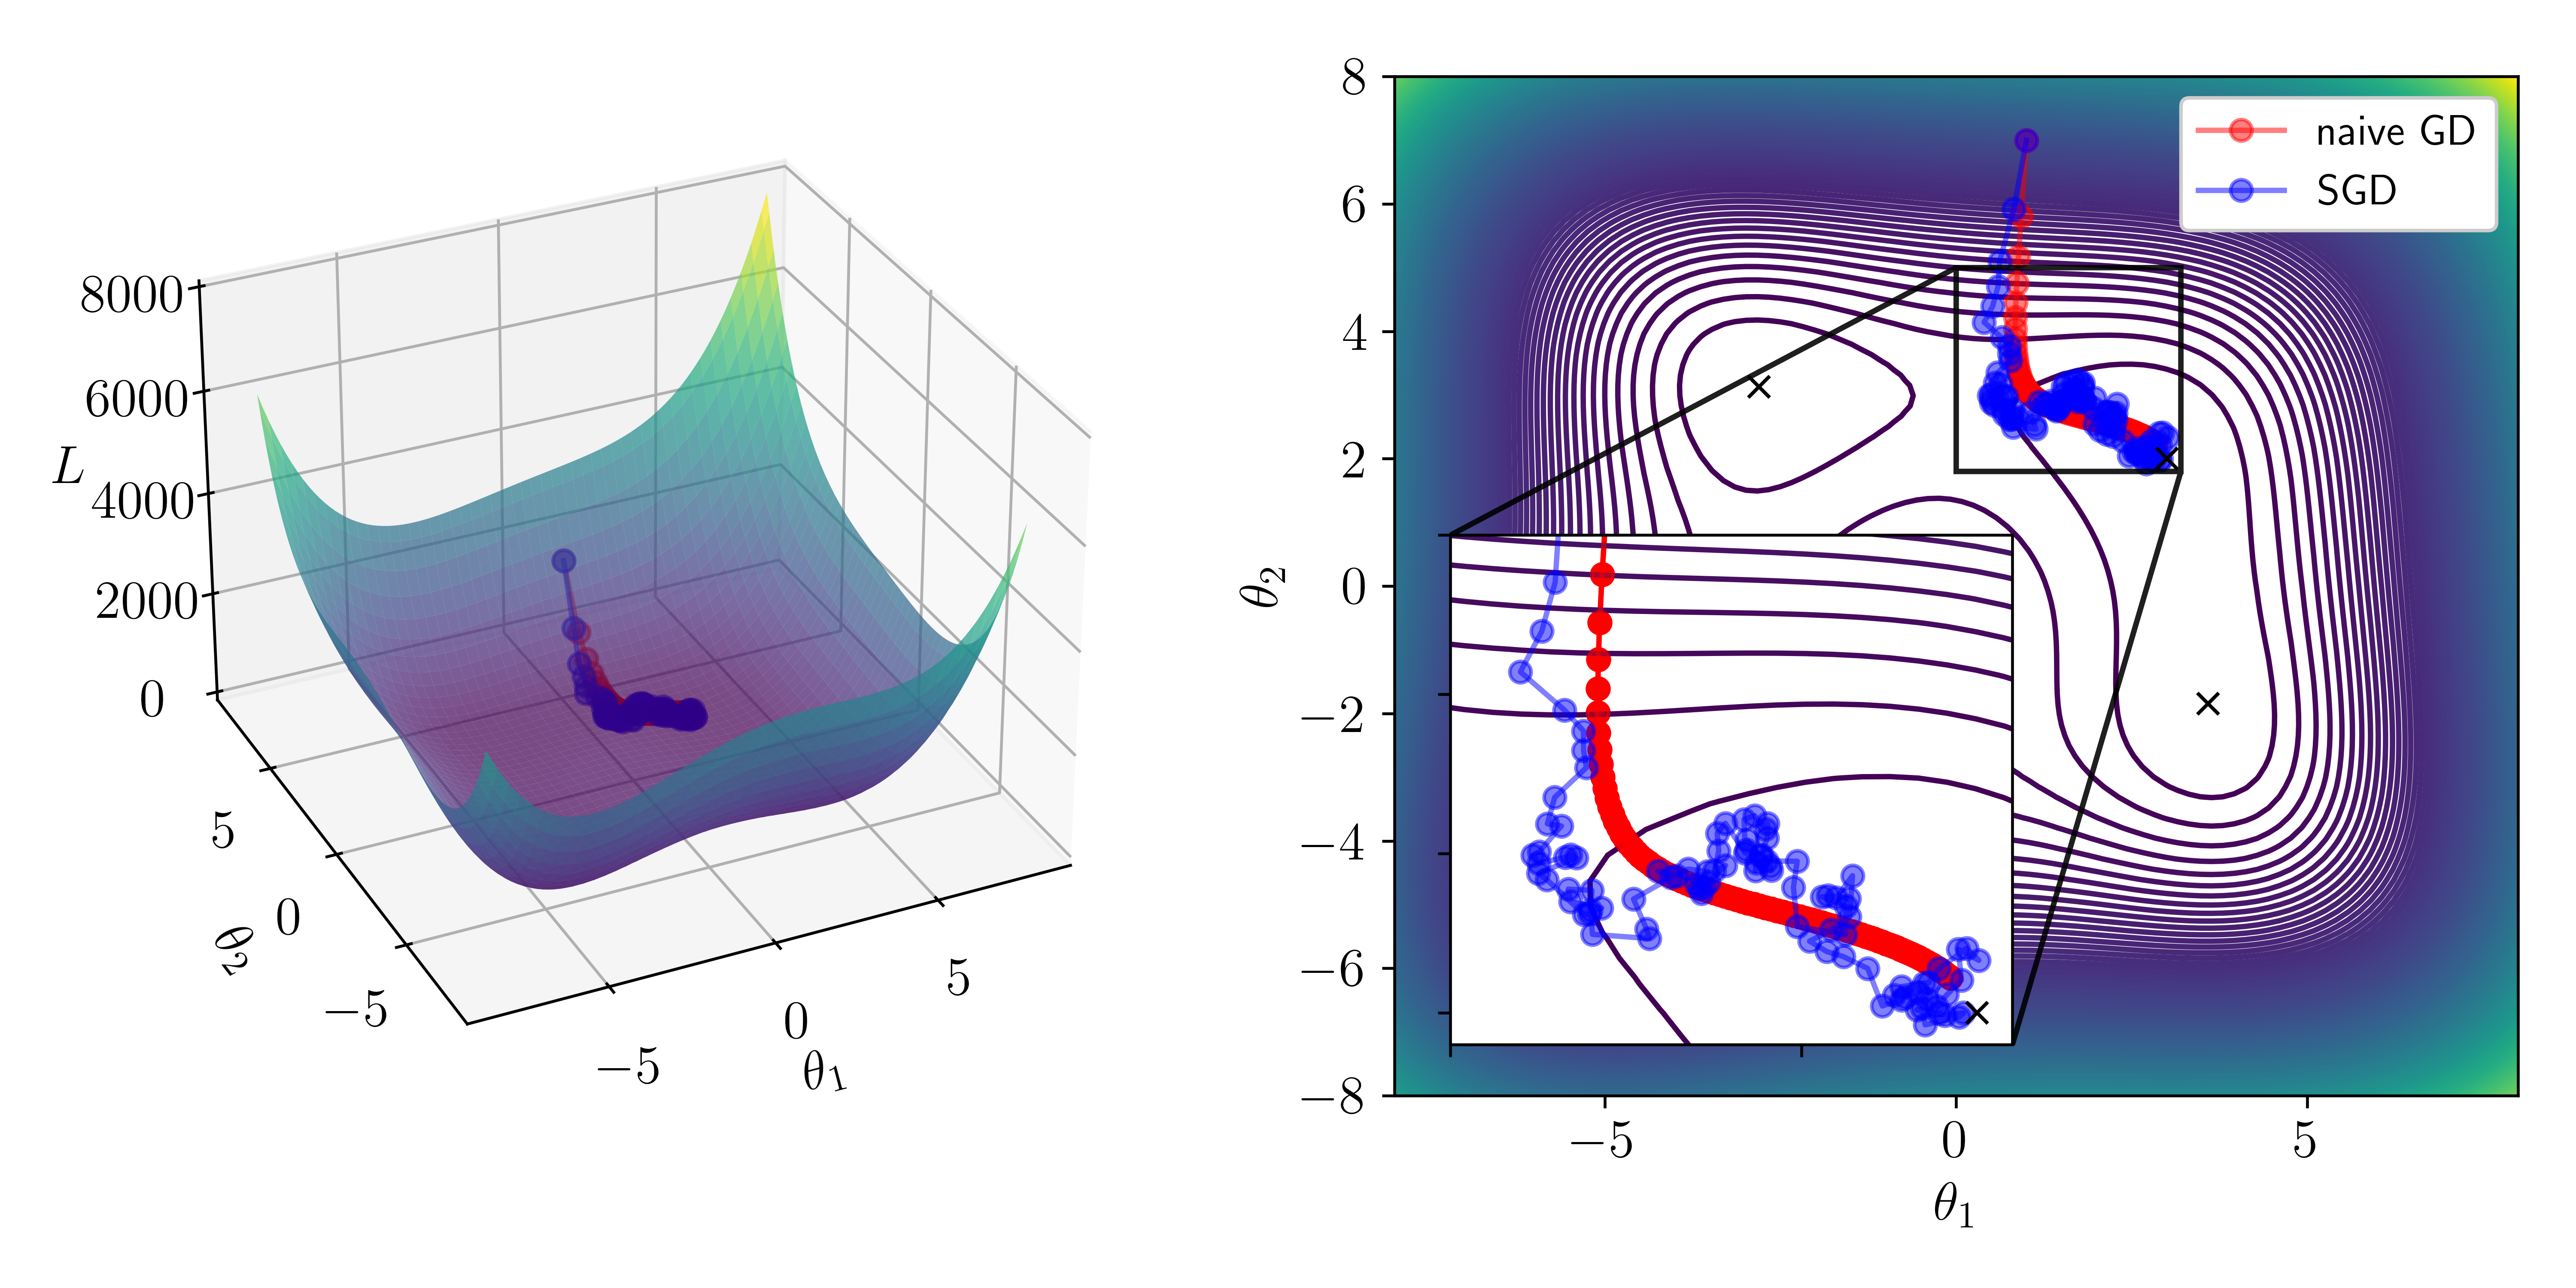
\includegraphics[width=\linewidth]{figs/stochastic_comparison.png}
    \caption{Comparison of SDG with naive GD on the Himmelblau function by a 3D plot (left), and a contour plot (right). Artificial noise selected from a normal distribtuion was added to the step direction to simulate stochastic effects. $1$ epoch, $100$ iterations, $\boldsymbol{\theta}^{(0)} = [1,7]$, with $\eta = 0.001$. Local minima are marked with $\times$. (Original)}
    \label{fig:enter-label}
\end{figure}

\section{Gradient Descent Methods}\label{sec:gradient-descent-methods}

The naive gradient descent algorithm introduced in Section~\ref{sec:optimization} has many limitations.

Perhaps the most obvious problem is that it is susceptible to critical points that are not the global minima of the loss function. Since $|\boldsymbol{\theta}|$ is usually very large, $L$ will have exceedingly many local minima and saddle points, any one of which may trap gradient descent.



\subsection{Momentum}
The \textbf{momentum} modification for gradient descent adds an ``inertia'' term, by also factoring the previous update into the current update. This is similar to the physical concept of momentum, where an object in motion tends to stay in motion.

Define the change in parameters for an update as $\mathbf{v}$, with $\mathbf{v}^{(0)} = 0$, as
\begin{equation}
    \mathbf{v}^{(t)} = \gamma \mathbf{v}^{(t-1)} - \eta \nabla L(\boldsymbol{\theta}^{(t)}),
\end{equation}
where $\gamma$ is a hyperparameter that determines the weight to which the previous movement is factored into the current movement. The parameters are then updated as
\begin{equation}
    \boldsymbol{\theta}^{(t+1)} = \boldsymbol{\theta}^{(t)} + \mathbf{v}^{(t)}.
\end{equation}
Note that gradient descent without momentum is just a special case of this, where $\gamma = 0$.

In effect, every movement is actually a weighted sum of all previous gradients, rather than just the most recent one.
\begin{equation}
    \mathbf{v}^{(n)} = \sum_{i=0}^{n} -\gamma^{n-i} \eta\nabla L(\boldsymbol{\theta}^{(i)}) = -\eta\nabla L(\boldsymbol{\theta}^{(n)}) - \gamma \eta\nabla L(\boldsymbol{\theta}^{(n-1)}) - \gamma^2 \eta\nabla L(\boldsymbol{\theta}^{(n-2)}) - \cdots
\end{equation}

\subsubsection{Nesterov Momentum}
In 1983, Russian mathematician Yurii Nesterov intrdouced a variant of momentum gradient descent by instead computing the gradient \textit{after} first applying the intertial term~\cite{nesterov_method_1983}.
\begin{equation}
    \mathbf{v}^{(t)} = \gamma \mathbf{v}^{(t-1)} - \eta \nabla L(\boldsymbol{\theta}^{(t)} + \gamma \mathbf{v}^{(t-1)}).
\end{equation}
This ``look-ahead'' method, usually called \textbf{Nesterov accelerated gradient (NAG)} or \textbf{Nesterov momentum}, allows the algorithm to be more responsive to the current gradient, and it is usually more effective than standard momentum. As such, Nesterov momentum is usually the default momentum implementation in software.
\begin{figure}[h]
    \centering
    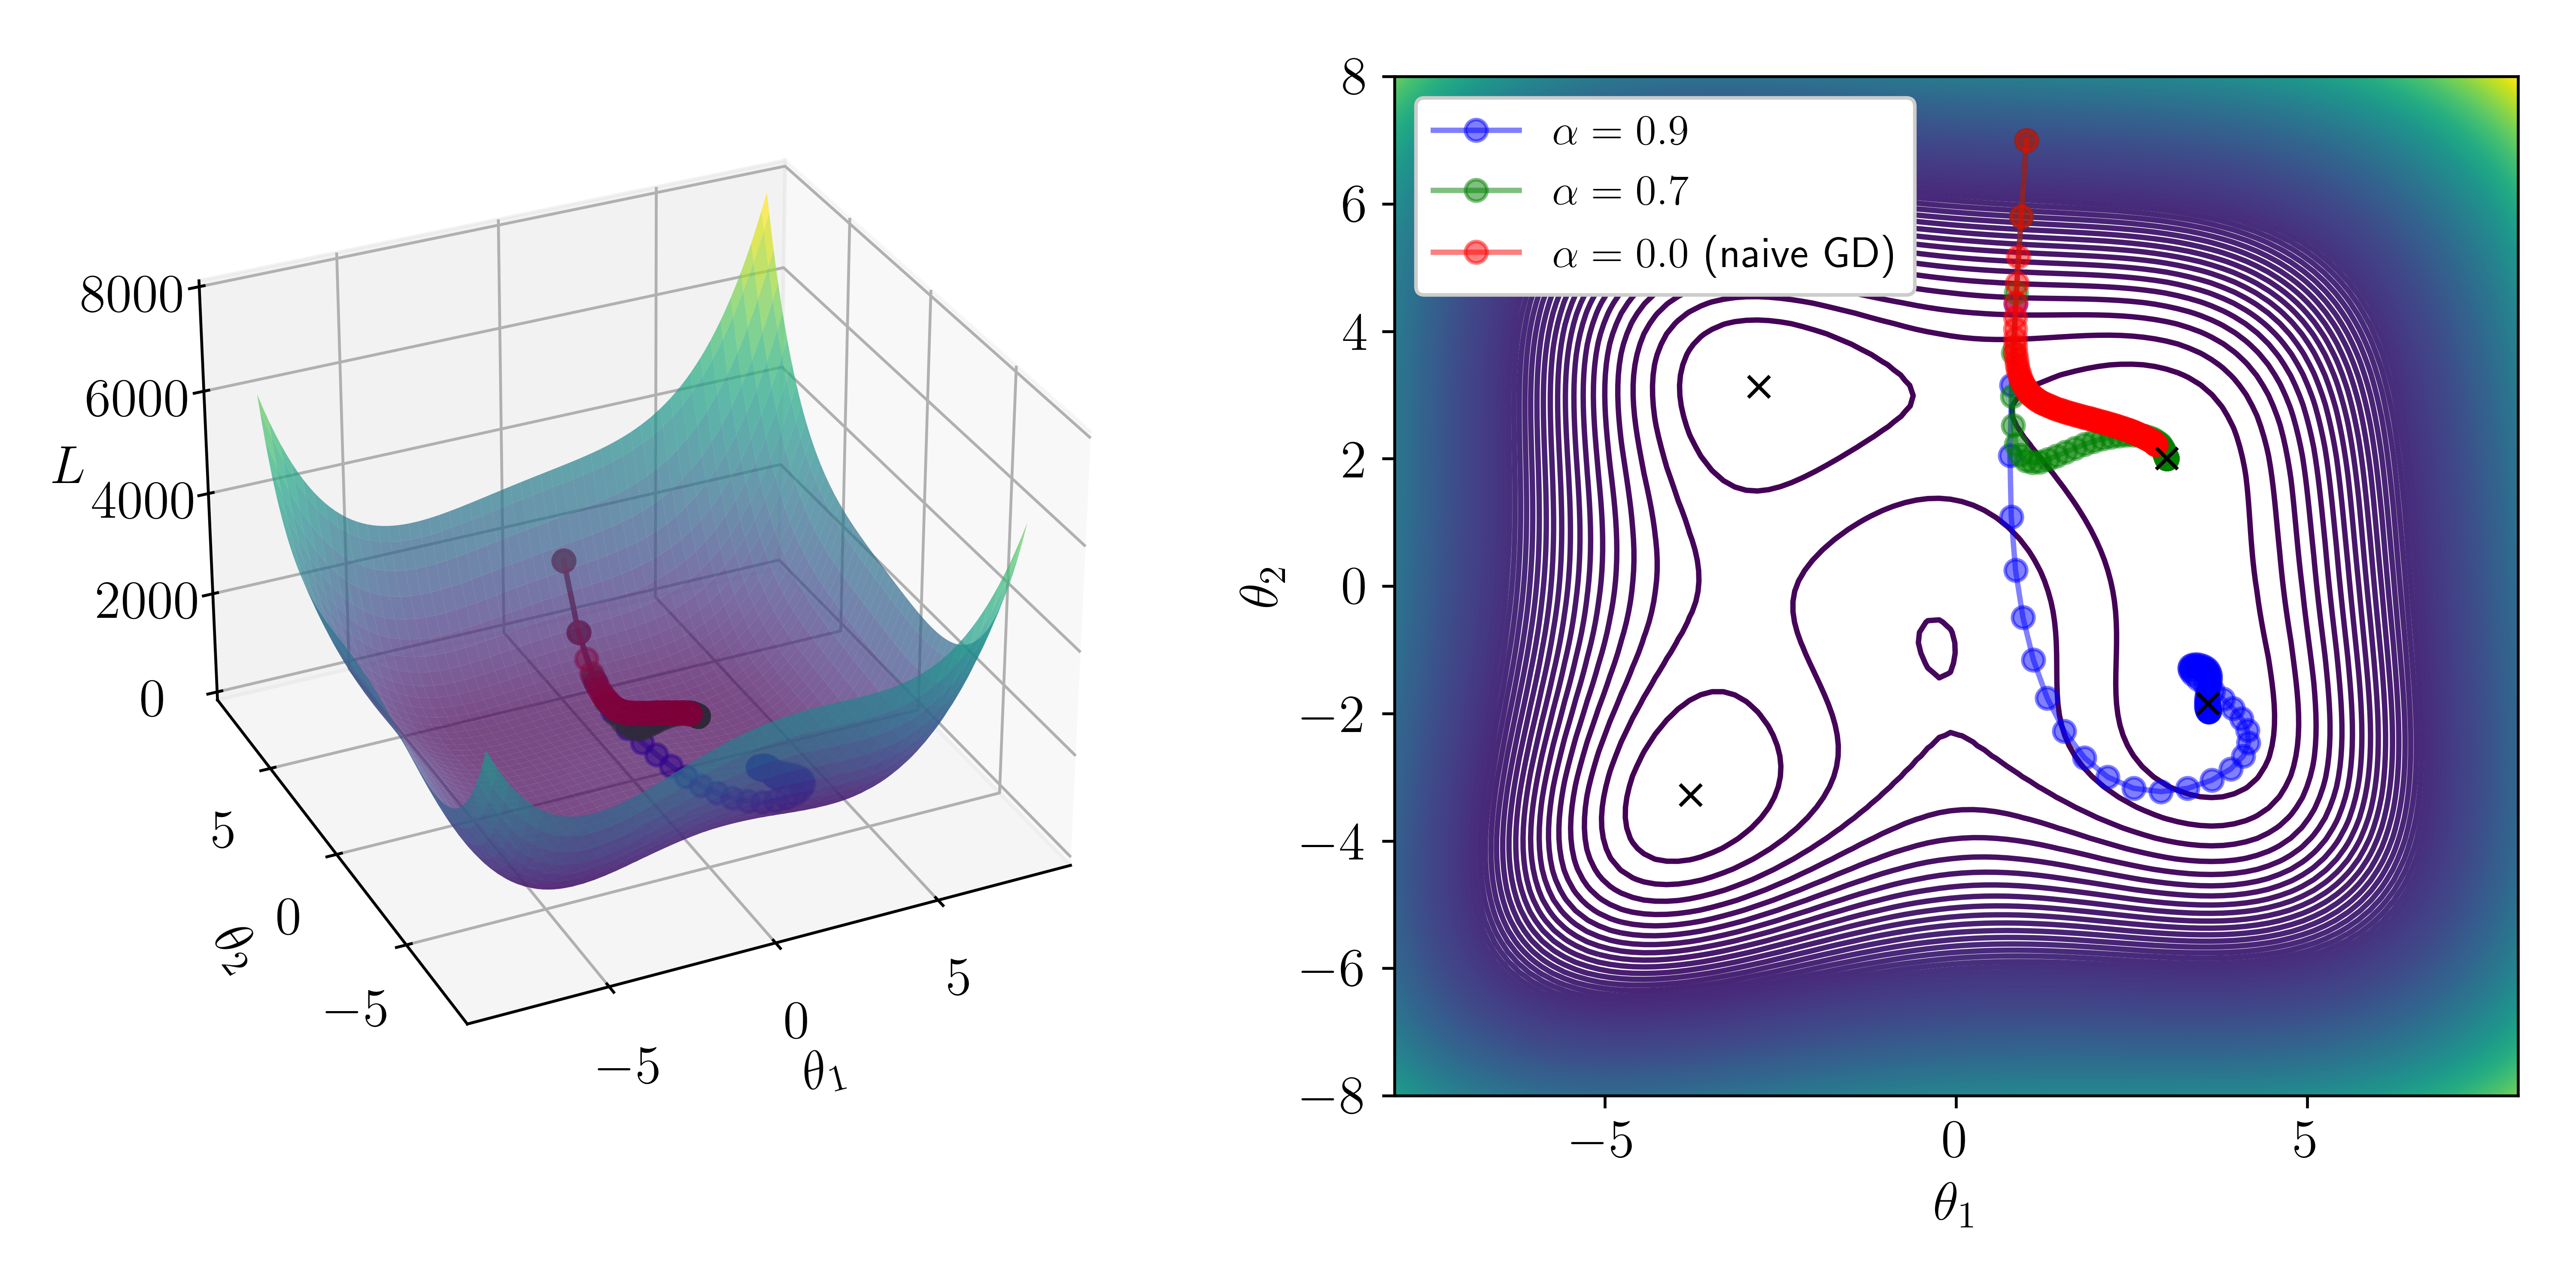
\includegraphics[width=\linewidth]{figs/nesterov_comparison.png}
    \caption{Comparison of Nesterov momentum optimizers on the Himmelblau function with various values of $\alpha$ visualized by a 3D plot (left), and a contour plot (right). $100$ iterations, $\boldsymbol{\theta}^{(0)} = [1,7]$, with $\eta = 0.001$. Local minima are marked with $\times$. (Original)}
    \label{fig:enter-label}
\end{figure}
Notice how momentum does not necessarily direct the model to the nearest local minima from the initial parameters. This has useful implications for training, as the model may be able to escape small local minima and saddle points, and it may be able to ``swing'' around large local minima to find a better minima elsewhere.

\subsection{Adaptive Learning Rate}
Since error surfaces are usually complex and non-uniform, a constant learning rate is not always ideal. For example, a small learning rate may be appropiate for a steep slope, but it may also be too small to make any progress on a relatively flat geometry. Conversely, a large learning rate may be appropriate for for flat geometries but may not converge to a minima on steep slopes. Error surfaces may also be anisotropic, where certain parameters are much more senesitive to changes than others.

Adaptive learning rates are a class of methods that introduce a variable $\sigma$ to be both time-dependent and parameter-dependent to allow for more flexibility in the learning process.
\begin{equation}
    \theta_{i}^{(t+1)} = \theta_{i}^{(t)} - \frac{\eta}{\sigma_i^t}\frac{\partial L}{\partial \theta_i^{(t)}}
\end{equation}

\subsubsection{Adagrad}
\textbf{Adapative Gradient Descent}, more commonly known as \textbf{Adagrad}, is a basic adapative learning rate method that sets $\sigma_i^{(t)}$ to be the sum of the squares of each iteration of the gradient with respect to the parameter $i$.
\begin{equation}
    \sigma_i^t = \sqrt{\sum_{j=0}^t {\left(\frac{\partial L}{\partial \theta_i^{(j)}}\right)}^2 + \epsilon}
\end{equation}
A very small $\epsilon \lll 1$ is included to prevent singularity problems when $\sigma_i^{(t)}$ is $0$.

\subsubsection{RMSprop}
$\sigma$ can only increase in Adagrad, which can cause problems if if the effective learning rate becomes too small. \textbf{RMSprop} is a modification of Adagrad that weights previous iterations of the gradient and the most recent gradient with a hyperparameter decay factor $\alpha$.
\begin{equation}
    \sigma_i^t = \sqrt{\alpha {(\sigma_i^{(t-1)})}^2 + (1-\alpha)\left(\frac{\partial L}{\partial \theta_i^{(t)}}\right)^2 + \epsilon}
\end{equation}
This allows RMSprop to be more flexible and responsive than Adagrad, slowing down when the gradient is large and speeding up when the gradient is small.
\subsubsection{Adam}
\textbf{Adaptive Moment Estimation}, or \textbf{Adam}, is a more advanced adaptive learning rate method that combines the ideas of momentum and RMSprop. It uses two decay factors, $\beta_1$ and $\beta_2$, to weight the previous iterations of the gradient and the squared gradient, respectively.

\cite{kingma_adam_2017}

read paper come back later

This algorithm is a standard in the field, and it is the default optimizer in many machine learning libraries, such as PyTorch.

\subsection{Learning Rate Scheduling}

The learning rate $\eta$ is a hyperparameter that is usually set to a constant value. However, it may be beneficial to instead define $\eta$ to vary with respect to iteration, $\eta^{(t)}$. This is called \textbf{learning rate scheduling}.
\begin{equation}
    \theta_{i}^{(t+1)} = \theta_{i}^{(t)} - \frac{\eta^{(t)}}{\sigma_i^t}\frac{\partial L}{\partial \theta_i^{(t)}}
\end{equation}
Typically, $\eta^{(t)}$ is set to decay as the number of iterations increases to prevent sudden explosions in step size after many iterations of small $\sigma$.

\subsubsection{Warmup}

lmao let the model warm up???

\section{Normalization}
So far, we have only discussed optimization methods that do not directly change the loss surface. By appling statistical \textbf{normalization}, we can make the loss sufrace easier to optimize, independently of the optimization method used.

\subsection{Feature Scaling}
\textbf{Feature scaling}, also called \textbf{data normalization} by some authors, is a technique that the features of the training data such that they are around the same magnitude. This as a variety of benefits, such as faster convergence gradient descent convergence, and in general, greater stability in training.

A common method is \textbf{standardization}, where features are normalized component-wise with their z-score with respect to the training data.
\begin{equation}
    \tilde{x}_i = \frac{x_i - \mu_i}{\sigma_i}
\end{equation}
Or, with vectors,
\begin{equation}
    \tilde{\mathbf{x}} = (\mathbf{x} - \boldsymbol{\mu}) \oslash \boldsymbol{\sigma}
\end{equation}

\subsection{Activation Normalization}
In the case of deep learning, normalization can also be applied to the activations of a layer.

\subsubsection{Batch Normalization}
\textbf{Batch normalization} (BatchNorm) is a very common implementation of activation normalization, applied before the actiavation function of a layer. BatchNorm takes advantage of the parallel computafortion of features within a batch and interleaves standardization simultaneously with the forward pass of the network.

insert figure here

Since normalization with z-scores moves the mean to $0$, this introduces some model bias. Parameters $\boldsymbol{\beta}$ and $\boldsymbol{\gamma}$ are introduced to get rid of this bias. They are \textit{not} hyperparameters and can be learned by the network. It is possible that these parameters will reintroduce disparities in magnitude, but they are usually initialized with values of $\mathbf{1}$ and $\mathbf{0}$ and only change the scaling slowly.

In testing, $\boldsymbol{\mu}$ and $\boldsymbol{\sigma}$ are replaced with moving averages, as it is infeasible to wait around for a full batch of data.

It is still debated why exactly BatchNorm is so effective, but the prevailing hypothesis is that it has the effect of smoothing the loss surface, making it easier to optimize.
\cite{ioffe_batch_2015}\cite{ioffe_batch_2017}\cite{santurkar_how_2019}

\section{Classification}\label{sec:classification}
Some tasks require a model to classify an input into one of a finite number of classes. Perhaps the most well known example is identifying handwritten digits from the MNIST dataset. In such cases, it is far from optimal to represent classes as scalar value features to train towards. Instead, classes are usually represented as one-hot vectors, where the index of the class is set to $1$, and all other indices are set to $0$.
\begin{equation}
    \mathbf{y} = \begin{bmatrix}
        0 \\
        1 \\
        0 \\
        0
    \end{bmatrix}
\end{equation}
\subsection{Softmax}
The output vector in classification is usually passed through the \textbf{softmax} function. The softmax function is a generalization of the sigmoid/logistic function to vector values, mapping all vectors to be wthin the unit hypercube. The softmax function is useful for classification problems, as it normalizes the output of a model to be a probability distribution over the classes, where the sum of all components is $1$. This is useful for many applications, such as when the output of a node is interpreted as a probability.

Formally defined, it is a function $\sigma\colon \mathbb{R}^K \to (0, 1)^K$, where $K > 1$, takes a vector $\mathbf{z} = (z_1, \dotsc, z_K) \in \mathbb{R}^K$ and computes each component of vector $\sigma(\mathbf{z}) \in (0, 1)^K$ with
\begin{equation}
\sigma(\mathbf{z})_i = \frac{e^{z_i}}{\sum_{j=1}^K e^{z_j}}\,.
\end{equation}
In other words, every component is exponentiated and then normalized by dividing with the sum of all exponentiated components.

The inputs to the softmax function are also called \textbf{logits}.

When implemented in code, the final normalized vector after being passed through the softmax function is then called by \textbf{argmax} to identify the index of the class with the highest probability, and thus the predicted class.
\begin{equation}
    \stackrel{\mbox{penultimate activation/logits $\mathbf{z}$}}{\begin{bmatrix}
        1.2 \\
        0.3 \\
        3.0 \\
        -0.9 \\
    \end{bmatrix}}
    \xrightarrow{\text{softmax}}
    \stackrel{\mbox{final layer probablilities $\sigma({\mathbf{z}})$}}{\begin{bmatrix}
        0.13 \\
        0.05 \\
        0.80 \\
        0.02 \\
    \end{bmatrix}}
    \xrightarrow{\text{argmax}}
    \stackrel{\mbox{identified class $\mathbf{y}$}}{\begin{bmatrix}
        0 \\
        0 \\
        1 \\
        0 \\
    \end{bmatrix}}
\end{equation}

\subsection{Cross Entropy Loss}

Recall the formula for the ubiquitous MSE loss for vector outputs.
\begin{equation}
L = \frac{1}{N}\sum \left(\sum_i (\hat{y}_i-y'_i)^2\right)
\end{equation}
For classification purpose, another loss called \textbf{cross entropy} is more commonly used instead, often paired with softmax. Minimizing cross entropy is equivalent to maximizing likelihood, for various information theory reasons. \url{https://www.youtube.com/watch?v=fZAZUYEeIMg}
\begin{equation}
L = \frac{1}{N}\sum \left(-\sum_i \hat{y}_i \ln y'_i\right)
\end{equation}
Note that $\ln y'_i$ is always negative because $y'$ is the output of the softmax, and thus the term inside the parentheses is always positive.

Cross entropy allso usually gives smoother loss surfaces compared to MSE for classification problems.

\chapter{Reinforcement Learning} % make all of this chapter more mathmatically rigorous
So far, we have only discussed ML techniques that are \textbf{supervised}, where the model is trained on a dataset with labels directing the model on what the desired output should be. The task of labeling is often done manually by a human, which is often infeasible or impractical for many applications. Sometimes, even humans may not even know what the best answer is.

The framework of \textbf{reinforcement learning (RL)} is a class of ML techniques that do not require labeled data, and thus are generally unsupervised. Instead, RL models learn by interacting with an environment, and receiving feedback in the form of rewards or penalties. The goal of an RL model is to learn a \textbf{policy} that maximizes the expected reward over time.

\begin{figure}[h]
    \centering
    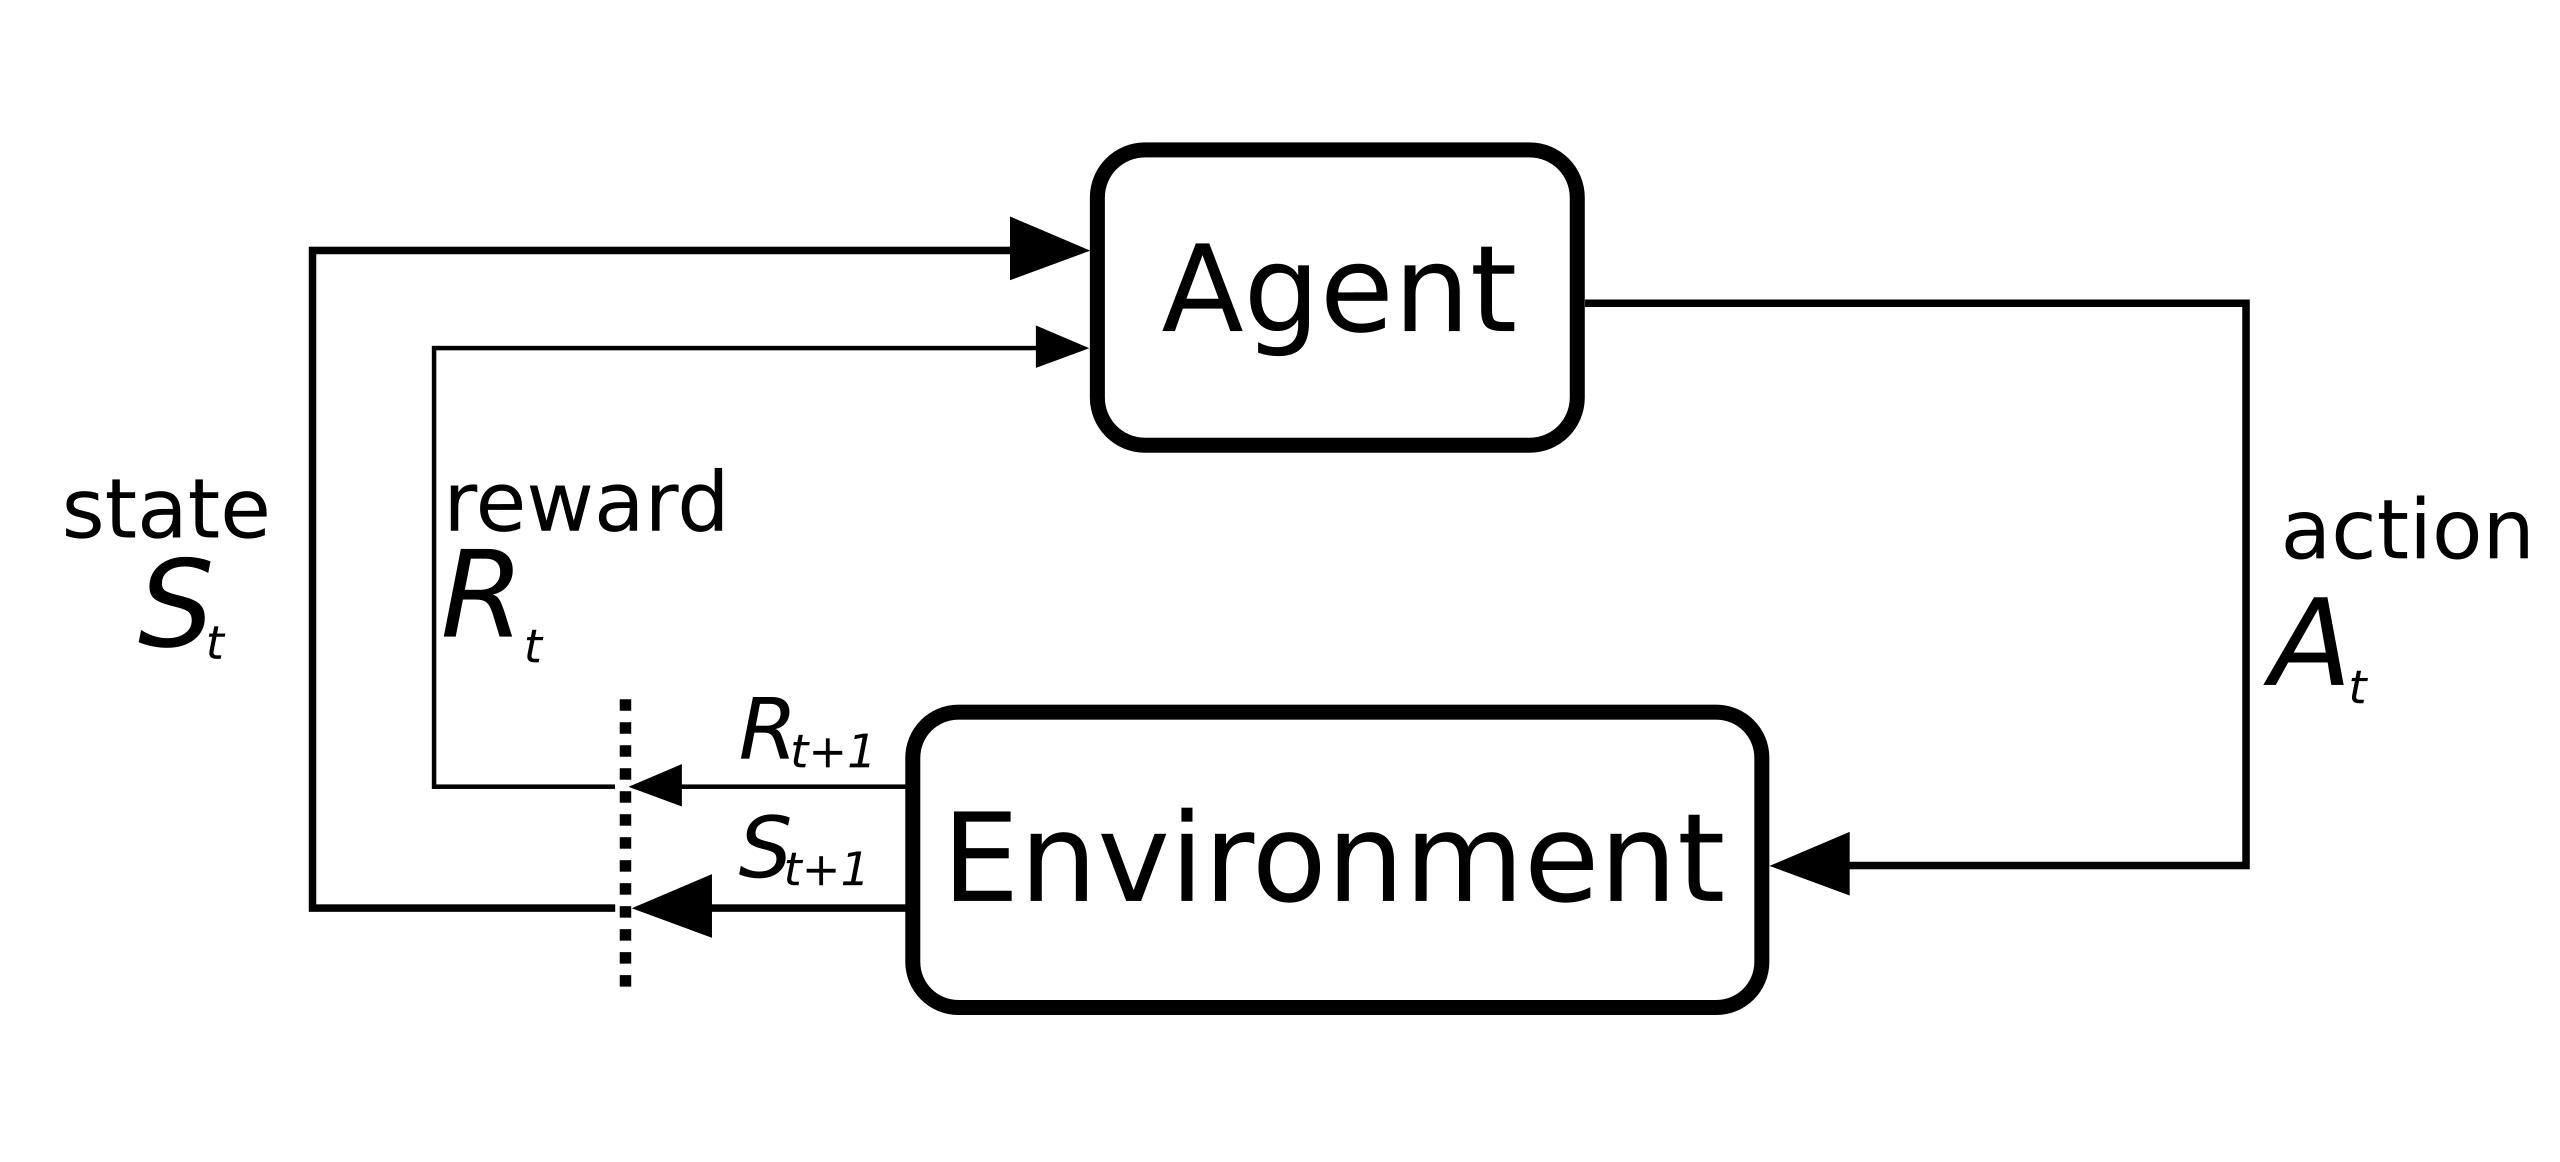
\includegraphics[width=0.5\linewidth]{figs/RL_schematic.png}
    \caption{\cite{commons_filemarkov_2023}}
    \label{fig:enter-label}
\end{figure}

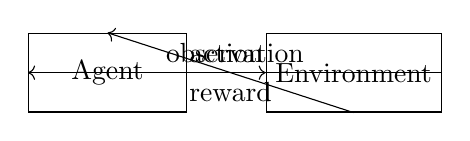
\begin{tikzpicture}
    \node (agent) [draw, rectangle, minimum width=2cm, minimum height=1cm] {Agent};
    \node (env) [draw, rectangle, minimum width=2cm, minimum height=1cm, right=of agent] {Environment};

    \draw[->] (agent.east) -- node[above] {action} (env.west);
    \draw[->] (env.east) -- node[above] {observation} (agent.west);
    \draw[->] (env.south) -- node[below] {reward} (agent.north);
\end{tikzpicture}


In RL, there are two main components: the \textbf{agent} and the \textbf{environment}. The agent is a model that takes in observations from the environment and outputs actions.  The environment then judges the action and returns a reward.

\section{Markov Decision Processes (MDPs)}

A \textbf{Markov descision process} (MDP) is a mathematical framework that can be used to model decisionmaking in a RL agent. MDPs are generalizations of \textbf{Markov chains}, which are stochastic processes that are \textbf{Markovian}, meaning that the future state of the process only depends on the current state, and not on any previous states. In other words, the future is independent of the past given the present; there is no hysteresis. Note that this does not mean that Markovian processes are deterministic.

Formally, an MDP is defined by a tuple $(\mathcal{S}, \mathcal{A}, P, R, \gamma)$, where:
\begin{itemize}
    \item $\mathcal{S}$, the \textbf{state space}, is the set of all possible states of the agent, which corresponds to the observations that the agent receives from the environment.
    \item $\mathcal{A}$, the \textbf{action space}, is the set of all possible actions that the agent can take.
    \item $\mathcal{P}$, the \textbf{transition function}, outputs the probability of transitioning from one state to another via a specific action.
    \item $\mathcal{R}$, the \textbf{reward function}, outputs the reward received by the agent after transitioning from one state to another given a specific action.
    \item $\gamma \in [0,1]$, the \textbf{discount factor}, is a hyperparameter that determines how much the agent should care about future rewards.
\end{itemize}



\begin{figure}[h]
    \centering
    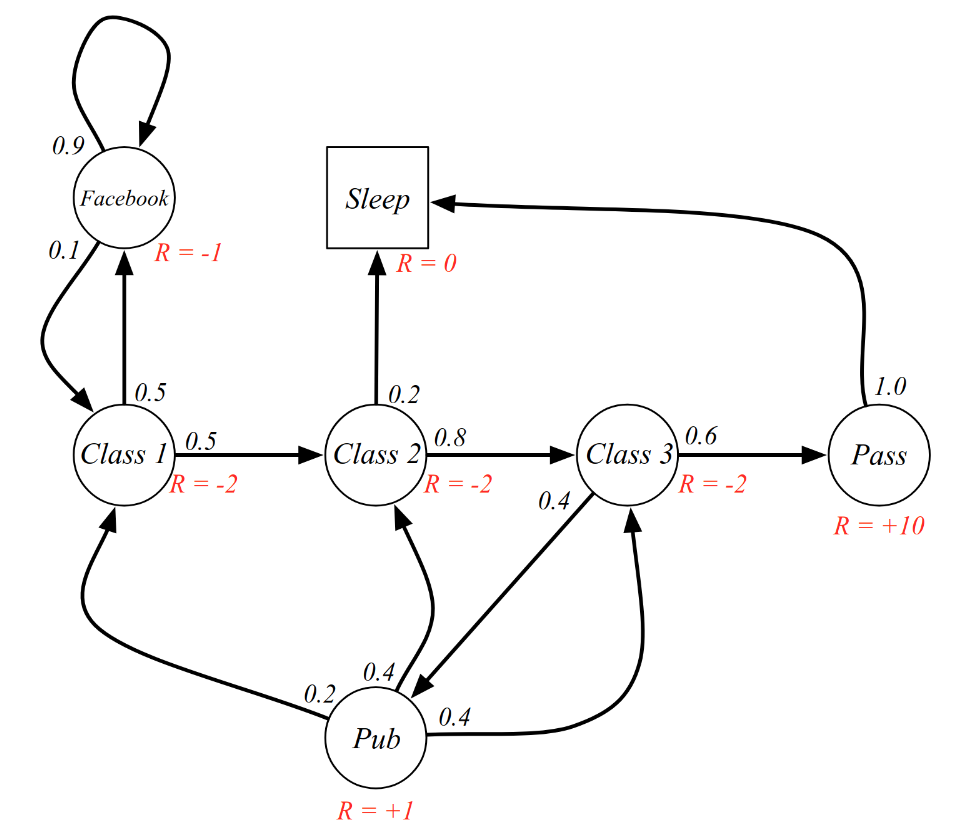
\includegraphics[width=0.7\linewidth]{figs/mdp.png}
    \caption{Reprinted from \cite{silver_lectures_2015}. Gotta make one of my own lol.}
    \label{fig:enter-label}
\end{figure}

\subsection{Episodes and Trajectories}
An \textbf{episode} is a single session of the agent in the environment, starting from an initial state $s_0$ and ending when the agent reaches a terminal state $s_T$. The agent interacts with the environment by taking actions $a_t$ and receiving rewards $r_t$ at each time step $t$ according to $\mathcal{R}$. The specific sequence of states, actions, and rewards that the agent experiences during an episode is called a \textbf{trajectory}.

\begin{equation}
    \tau = (s_0, a_0, r_0, s_1, a_1, r_1, \ldots, s_T, a_T, r_T)
\end{equation}

A set of trajectories experienced by an agent may be collectively considered as $\mathcal{D}$ in notation. Typically, $\mathcal{D}$ is the training data used for optimizing the agent.

\subsection{Policies}

The \textbf{policy} $\pi(s, a): \mathcal{S} \times \mathcal{A} \to [0,1]$ is a function that outputs the probability of taking action $a$ in state $s$.
\begin{equation}
    \pi(a | s) = \mathbb{P}(a_t = a | s_t = s)
\end{equation}
Equivalently, the policy can be thought of as a function that maps from the state space to a probability distribution over the action space.

Recall the universal approximation theorem from Section~\ref{sec:nn}. Since $\pi$ is a function that maps from the state space to a probability distribution over the action space, it can be approximated by a classification neural network. An optimal $\pi$ is almost always highly complex and non-linear, and thus for most applications of RL, $\pi$ is represented by a neural network. The neural network then called the \textbf{policy network} of the agent.

The pairing of deep learning with RL is called \textbf{deep reinforcement learning} (DRL). We will mainly discuss RL concepts and methods in the context of DRL, as it is widespread in the field of robotics, however it is important to note that RL is not limited to DRL\@. In fact, many of the RL methods discussed in this article can be applied to non-neural network policies as well.

\subsubsection{Evaluating Policies}
The goal of the agent is to learn a policy that maximizes the expected reward over time. How can we encapuslate this idea mathematically?

Recall that the environment returns a reward according to $R$ each time the agent takes an action $a_t$. It would be unreasonable to assume that the immediate reward for that action is the only thing that matters. An action may have long-term consequences that affect the future rewards of the agent. Therefore rather than only considering a specific $r_t$, we consider the \textbf{discounted return} $G$ as the metric to judge an action.
\begin{equation}
    G_t = r_t + \gamma r_{t+1} + \gamma^2 r_{t+2} + \cdots = \sum_{k=0}^{\infty} \gamma^k r_{t+k}
\end{equation}
$G$ can be defined on a trajectory $\tau$ as
\begin{equation}
    G(\tau) = \sum_{t=0}^{T} \gamma^t r_t.
\end{equation}

The \textbf{expected return} $J_\pi$ of a policy $\pi$ is then formally defined as the expected value $G$ over all possible trajectories that the agent may take.
\begin{equation}\label{eq:expected-return}
    J_\pi = \mathbb{E}_\pi[G(\tau)] = \int_{\tau} G(\tau)\mathbb{P}_\pi(\tau)\ d\tau.
\end{equation}
This value, $J_\pi$, is the value that we want to maximize to optimize the policy $\pi$.

Additionally we may define two other closely related functions, the \textbf{state-value function} $V_\pi(s): \mathcal{S} \to \mathbb{R}$ defined as the expected discounted return of the agent at state $s$,
\begin{equation}
    V_\pi(s) = \mathbb{E}_\pi[G_t | s_t = s],
\end{equation}
and the \textbf{action-value function} $Q_\pi(s, a): \mathcal{S} \times \mathcal{A} \to \mathbb{R}$ defined as the expected discounted return of the agent at state $s$ and taking action $a$,
\begin{equation}
    Q_\pi(s, a) = \mathbb{E}_\pi[G_t | s_t = s, a_t = a].
\end{equation}
Note the following relationship between the two functions,
\begin{equation}
    V_\pi(s) = \sum_a \pi(a | s) Q_\pi(s, a).
\end{equation}

\subsubsection{Bellman Equation}

\subsubsection{Learning Policies}

\subsection{Continuous State and Action Spaces}
Up to this point, our notation has been limited to discrete state and action spaces. It is important to take note that for many applications $\mathcal{S}$ and $\mathcal{A}$ may be continuous spaces, such as the position and velocity of a robot arm, or the torque to apply to a joint. It is rather easy in most cases to extend the concepts that we have discussed to the continuous case: replacing sums with integral, probabilities with probability density functions, and so on. So, we will not go into much detail here about the specific nuances between discrete and continuous domains, just keep in mind that there may be some abuses of notation here and there.

\section{Policy Gradient}
\textbf{Policy gradient} methods are a class of RL algorithms that learn a policy by directly optimizing the expected return $J_\pi$. This is typically accomplished by parameterizing the policy $\pi$ with $\boldsymbol{\theta}$ and then using gradient descent/ascent to optimize $J_\pi$ with respect to $\boldsymbol{\theta}$. Note that this is exactly the same as the optimization problem we have discussed in the previous chapter. In fact, in DRL, the parameters of the policy \textit{are precisely} the parameters of its neural network.

\subsection{Policy Gradient Theorem}
The \textbf{policy gradient theorem} (see proof in Appendix~\ref{sec:policy-gradient-theorem-proof}) states that the gradient of $J_\pi$ with respect to the parameters $\boldsymbol{\theta}$ can be expressed as
\begin{equation}\label{eq:policy-gradient-theorem}
    \nabla_{\boldsymbol{\theta}} J_\pi =  \mathbb{E}_\pi\left[G(\tau) \sum_{t=0}^{T} \nabla_{\boldsymbol{\theta}} \log \pi_{\boldsymbol{\theta}}(a_t | s_t)\right],
\end{equation}
where the summation represents all pairs of $(s_t, a_t)$ in a trajectory.
This is a important result, as it allows us to compute the gradient of $J_\pi$, and thus optimizing $\boldsymbol{\theta}$, without having to compute the state-value function $V_\pi$. Inaddition, policy gradient methods are \textbf{model-free} methods, as they do not require any knowledge of the environment, its associated value functions or the transition function. The theorem only presupposes that $\pi_{\boldsymbol{\theta}}$ is differentiable, which is a reasonable assumption for almost all neural networks.

In practice, the right-hand side of the equation is estimated by sampling trajectories from the environment in a Monte Carlo fashion, and then computing the average over all sampled trajectories.
\begin{equation}
    \nabla_{\boldsymbol{\theta}} J_\pi \approx \frac{1}{N} \sum_{i=1}^{N} G(\tau^{(i)}) \sum_{t=0}^{T} \nabla_{\boldsymbol{\theta}} \log \pi_{\boldsymbol{\theta}}(a_t^{(i)} | s_t^{(i)})
\end{equation}

\subsection{\texttt{REINFORCE}}

In 1992, Ronald J. Williams introduced the basic \texttt{REINFORCE} algorithm, which uses an even simpler version of the policy gradient theorem in combination with sampling trajectories in a Monte Carlo manner.~\cite{williams_simple_1992}
\begin{algorithm}
    \caption{\texttt{REINFORCE} with policy $\pi_{\boldsymbol{\theta}}$, learning rate $\eta$, and $N$ episodes.}\label{alg:REINFORCE}
    \begin{algorithmic}[1]
        \State Initialize parameters $\boldsymbol{\theta}$
        \For{$i = 1, \ldots, N$}
            \State Play episode $i$
            \State $\tau^{(i)} \leftarrow (s_0^{(i)}, a_0^{(i)}, r_0^{(i)}, \ldots, s_T^{(i)}, a_T^{(i)}, r_T^{(i)})$
            \For{$t = 0, \ldots, T$}
                \State $G_t^{(i)} \leftarrow \sum_{k=0}^{T} \gamma^k r_{t+k}^{(i)}$
                \State $\nabla_{\boldsymbol{\theta}} J_\pi \leftarrow G_t^{(i)} \nabla_{\boldsymbol{\theta}} \log \pi_{\boldsymbol{\theta}}(a_t^{(i)} | s_t^{(i)})$
                \State $\boldsymbol{\theta} \leftarrow \boldsymbol{\theta} + \eta \nabla_{\boldsymbol{\theta}} J_\pi$
            \EndFor
        \EndFor \\
        \Return $\boldsymbol{\theta}$
    \end{algorithmic}
\end{algorithm}
Note that line \texttt{8} is equivalent to gradient descent on $-J_\pi$, which means that all the the optimization techniques that we have discussed in Section~\ref{sec:gradient-descent-methods} can be applied here, up to a difference in sign.

\subsection{Trust Region Policy Optimization (TRPO)}
\cite{schulman_trust_2015}


\subsection{Proximal Policy Optimization (PPO)}
\cite{schulman_proximal_2017}

\section{Actor-Critic Methods}
In contrast to policy gradient methods, \textbf{actor-critic} methods learns the state-value function $V_\pi$ directly. We define a \textbf{critic} as a seperate entity from the the agent, which also may be a neural network.

\subsection{Advantage Actor-Critic (A2C)}

\section{Q-Learning}

\section{Reward Shaping}
Some environments have very sparse rewards, such as playing chess or go, where the agent only receives a definitive reward at the end of the game based on whether it wins or loses. This is a problem for learning, as the agent have trouble associating the actions it took during the game with the final reward. This is an example of the \textbf{credit assignment problem}, which is the fundamental reason why RL is so difficult.

Thus, we may define additional rewards to guide the agent, by \textbf{reward shaping}. By applying domain knowledge, we can notice that certain actions are more likely to lead to a positive outcome, and assign a small reward for those actions, even if they are not inherent in the environment.

\subsection{Example: VizDoom}

VizDoom is a adaptation of the classic 1996 video game \textit{Doom} for use as a RL research environment~\cite{kempka_vizdoom_2016}. \textit{Doom} is a first-person shooter game where the player must navigate through a maze and defeat enemies. The game is highly complex, but rewards are sparse, as the player only receives a reward when they beat the level. Therefore, researchers introduce additional rewards for picking up medkits, killing enemies, and even just surviving and moving around.

\begin{figure}[h]
    \centering
    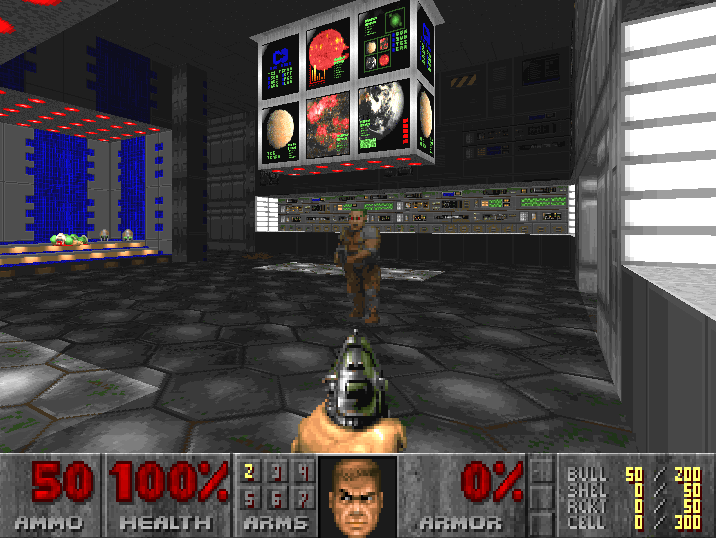
\includegraphics[width=0.5\linewidth]{figs/doom.png}
    \caption{Reprinted from~\cite{kempka_vizdoom_2016}.}
    \label{fig:enter-label}
\end{figure}

\subsection{Curiosity}
\textbf{Curiosity} is a form of intristic reward that incentivizes the agent to explore its environment and to encounter novel states. The idea behind curiosity is that increasing the seen state space of the agent will allow it learn a better policy, as it has a more complete understanding of the environment. When there are sparse extrinsic rewards, or even a complete absence of extrinsic rewards, curiosity can be effective for training an agent in such environments~\cite{pathak_curiosity-driven_2017}. This idea finds applications where the environment is not well defined and lacking of any obvious reward structure.

maybe put fig here?

\section{Imitation Learning}
In cases where an optimal or desired behavior is known, such as in the case of human demonstrations, it may be more efficient to train a model to imitate the behavior from an expert rather than learning from scratch. This is called \textbf{imitation learning}. Immitation learning is a form of supervised learning, where the model is trained on a dataset of demonstrations.

\textbf{Behavior cloning (BC)} is a form of imitation learning, where the policy network $\pi(a|s)$ simply learns from state-action pairs $(s, a)$ from expert demonstrations. This technique is very straightforward to implement but it is also very limited. For example, mismatches may occur when the learned policy is placed in an unfamiliar environment that was never reached by the expert. A simple analogy, is learning how to play soccer by watching Messi. You are not Messi. Messi will never make basic mistakes, but you will, and you will not know what to do in those situations.

\subsection{more methods look into them}

\subsection{Inverse Reinforcement Learning (IRL)}
In contrast to behavior cloning, \textbf{inverse reinforcement learning (IRL)} is a form of imitation learning where the model learns a reward function (usually in the form of a neural network) from expert demonstrations, rather than the expert policy. The learned reward function can then be used to train a from-scratch agent using standard RL methods.
\cite{arora_survey_2021}

\chapter{Robotic Systems and Control}

\section{Hutter, Lee, Hwangbo et al.\ and the ANYmal by ANYbotics}
Originally developed for the DARPA Robotics Challenge, the ANYmal is a quadrupedal robot developed by ANYbotics. It is a highly capable platform that has been used in a variety of applications, including search and rescue, inspection, and exploration.

Using deep reinforcement learning, Marco Hutter et al.\ trained the ANYmal to walk and navigate rather than using previous traditional pathfinding and trajectory optimization methods.

\cite{hutter_anymal_2016}

\begin{figure}[h]
    \centering
    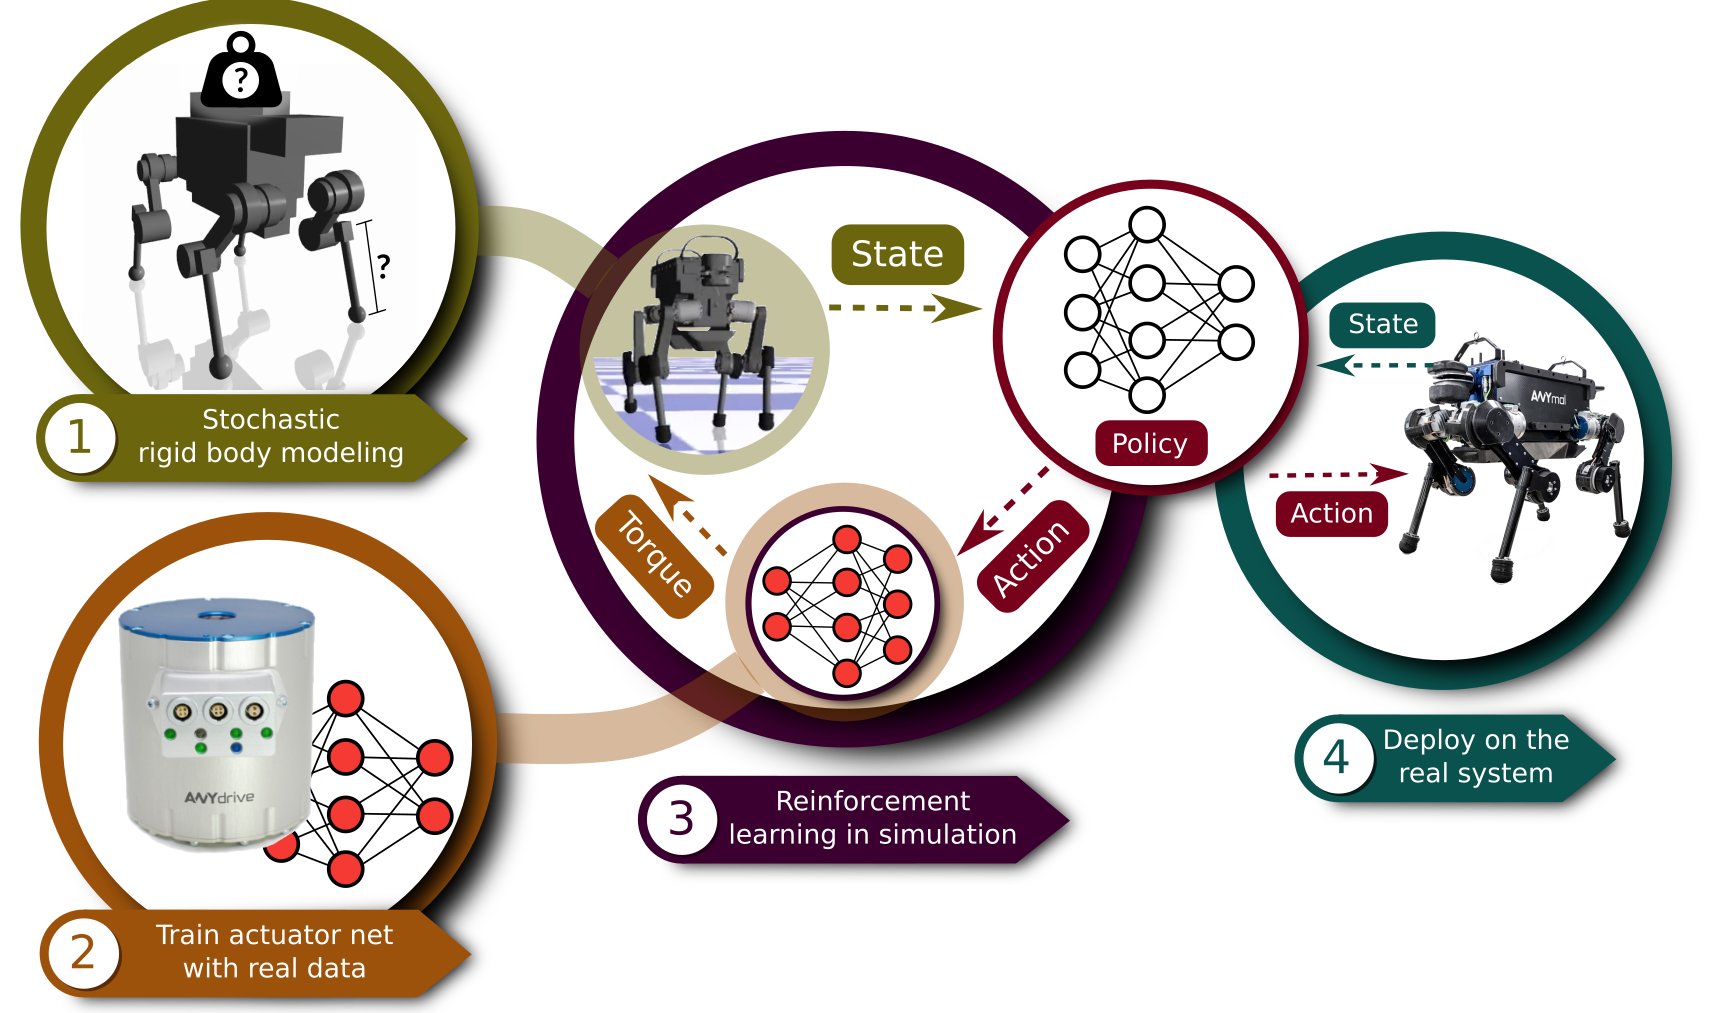
\includegraphics[width=\linewidth]{figs/anymal_RL.png}
    \caption{Repreinted from~\cite{hwangbo_learning_2019}.}
    \label{fig:enter-label}
\end{figure}

\begin{figure}[h]
    \centering
    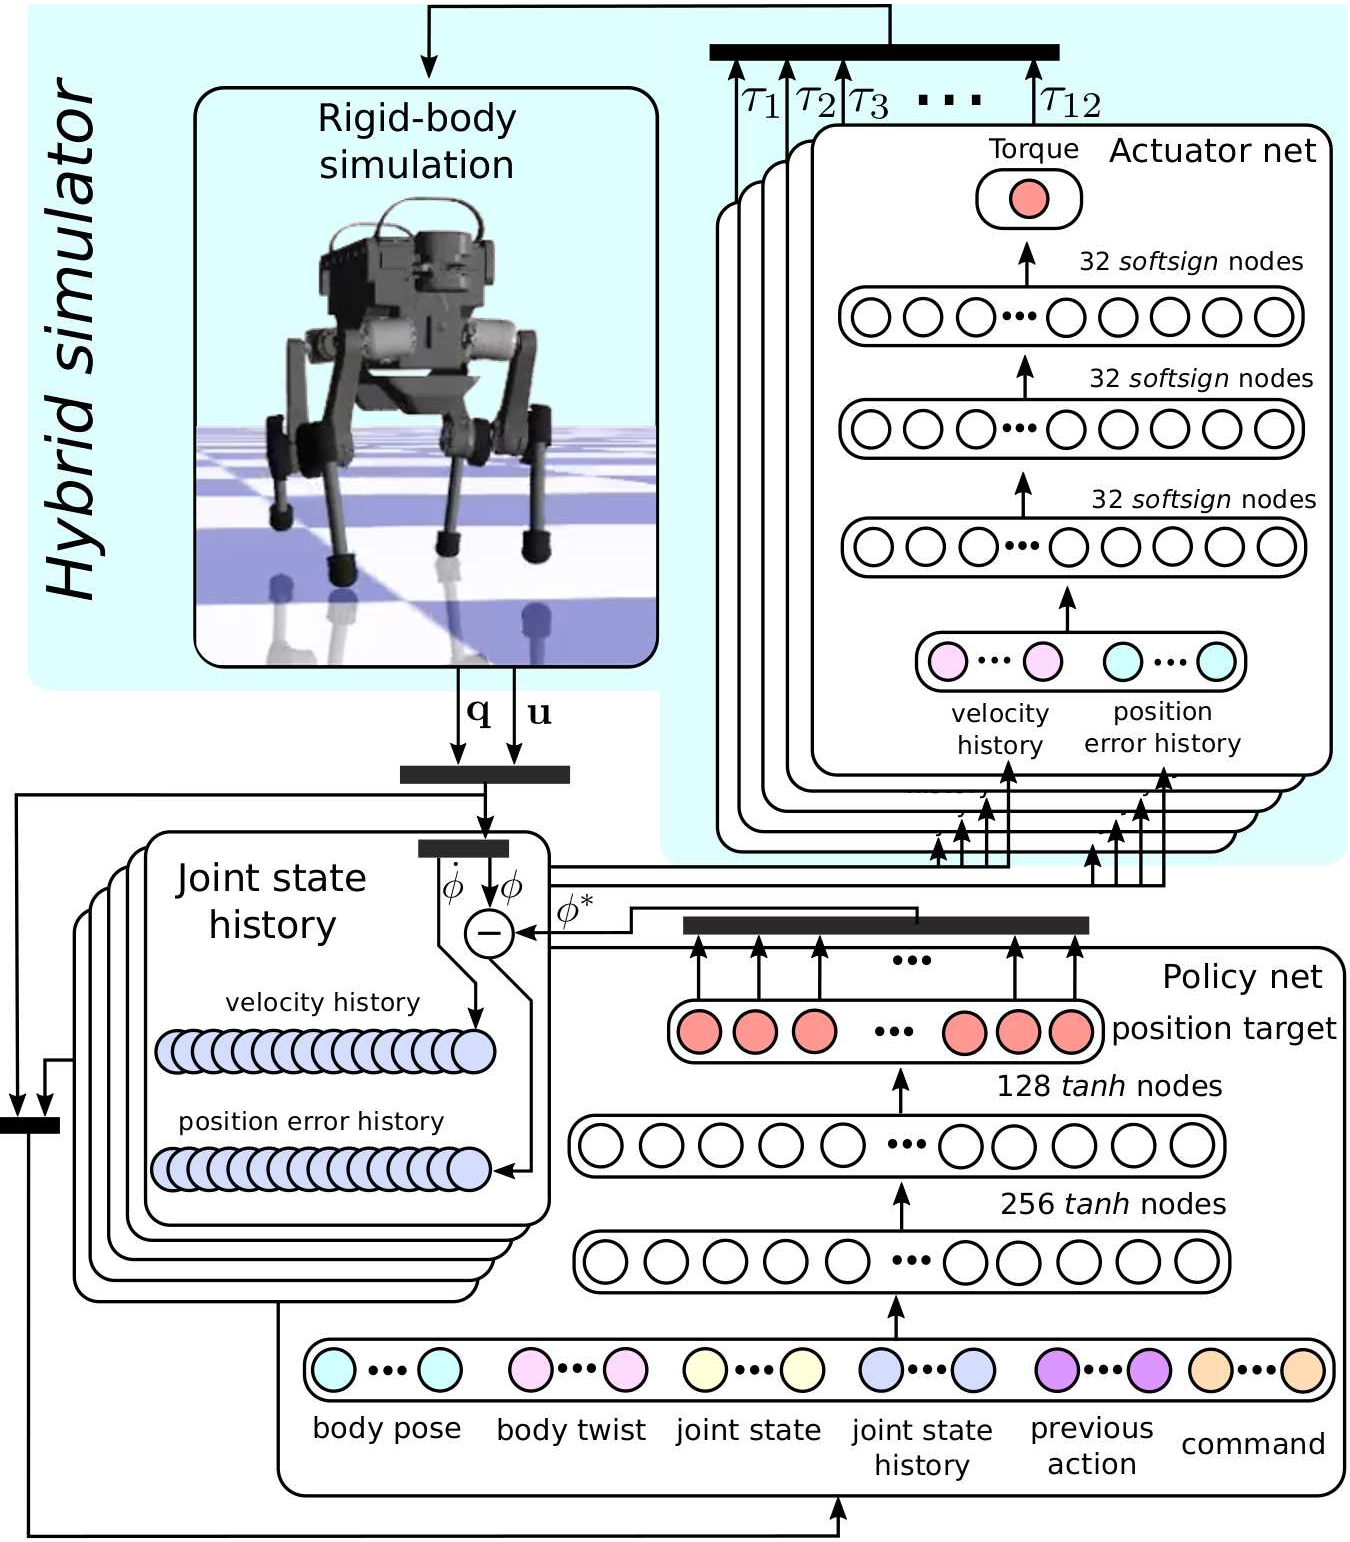
\includegraphics[width=0.5\linewidth]{figs/anymal_detailed.png}
    \caption{Reprinted from~\cite{hwangbo_learning_2019}.}
    \label{fig:enter-label}
\end{figure}

\begin{figure}[h]
    \centering
    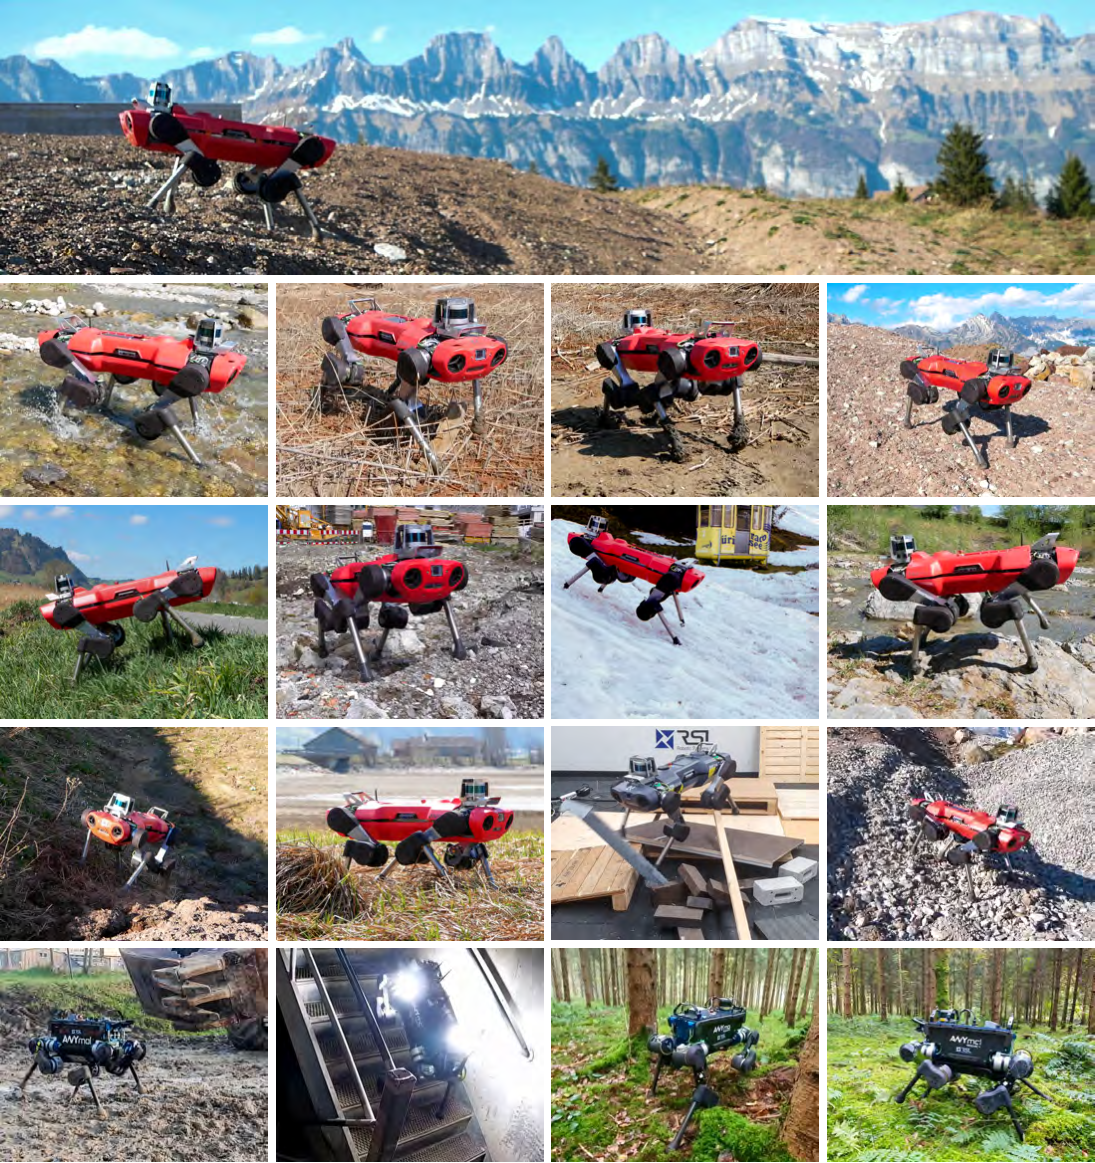
\includegraphics[width=\linewidth]{figs/figure1.pdf}
    \caption{Reprinted from~\cite{lee_learning_2020}.}
    \label{fig:enter-label}
\end{figure}

\begin{figure}[h]
    \centering
    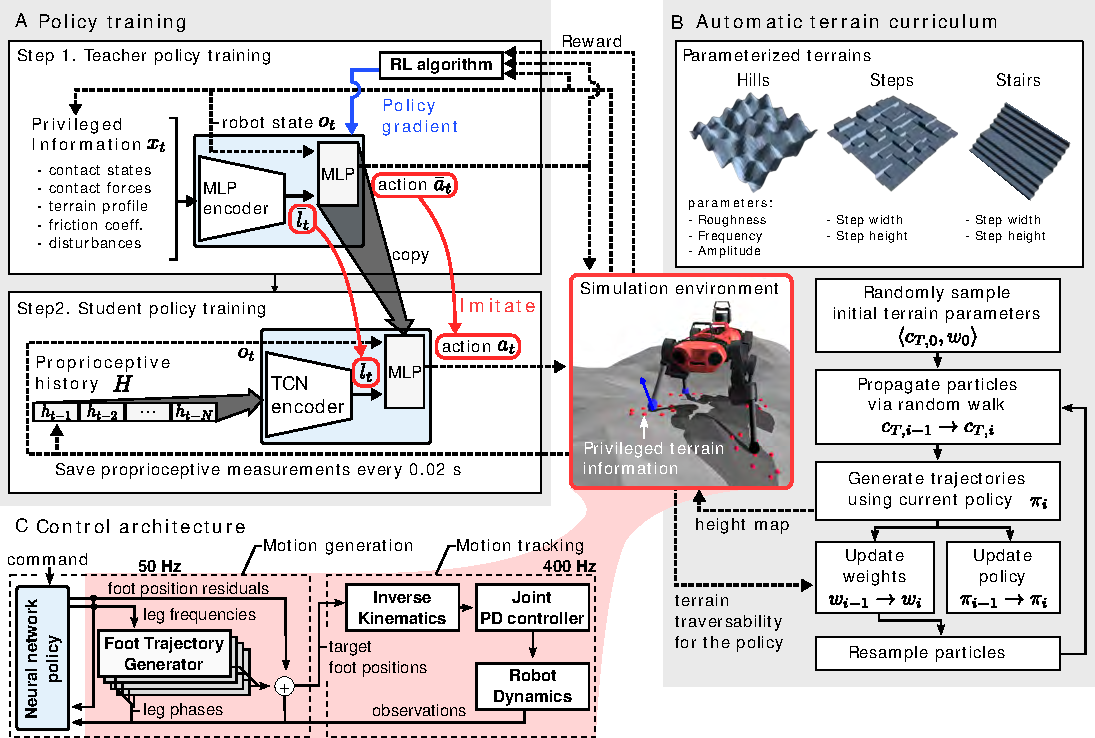
\includegraphics[width=\linewidth]{figs/figure4.pdf}
    \caption{Reprinted from~\cite{lee_learning_2020}.}
    \label{fig:enter-label}
\end{figure}

\cite{hutter_legged_2022}
\cite{lee_learning_2020}

\section{Luo et al.\ and Exoskeletons}
\cite{luo_reinforcement_2021}
\cite{luo_experiment-free_2024}


\section{more examples will go here}


\begin{appendices}
\chapter{Proofs}
\section{Policy Gradient Theorem (Equation~\ref{eq:policy-gradient-theorem})}\label{sec:policy-gradient-theorem-proof}
\begin{proof}
    By definition (Equation~\ref{eq:expected-return}), the expected return $J_\pi$ is defined as
    \begin{equation*}
        J_\pi = \mathbb{E}_\pi[G(\tau)] = \int_{\tau} G(\tau)\mathbb{P}_{\boldsymbol{\theta}}(\tau)\ d\tau.
    \end{equation*}
    Next, take the gradient with respect to the parameters $\boldsymbol{\theta}$ of the policy $\pi$ to both sides of the equation.
    \begin{align*}
        \nabla_{\boldsymbol{\theta}} J_\pi &= \nabla_{\boldsymbol{\theta}} \int_{\tau} G(\tau)\mathbb{P}_{\boldsymbol{\theta}}(\tau)\ d\tau \\
        &= \int_{\tau} G(\tau) \nabla_{\boldsymbol{\theta}} \mathbb{P}_{\boldsymbol{\theta}}(\tau)\ d\tau \tag{by Leibniz integral rule} \\
        &= \int_{\tau} G(\tau) \mathbb{P}_{\boldsymbol{\theta}}(\tau) \nabla_{\boldsymbol{\theta}} \log \mathbb{P}_{\boldsymbol{\theta}}(\tau)\ d\tau \tag{$\partial \log f(x) = \frac{1}{f(x)}\partial f(x)$} \\
        &= \mathbb{E}_{\boldsymbol{\theta}}\left[G(\tau) \nabla_{\boldsymbol{\theta}} \log \mathbb{P}_{\boldsymbol{\theta}}(\tau)\right] \tag{by the definition of expectation} \\
        &= \mathbb{E}_{\boldsymbol{\theta}}\left[G(\tau) \nabla_{\boldsymbol{\theta}} \log \left(\prod_{t=0}^{T} \pi_{\boldsymbol{\theta}}(a_t | s_t)\right)\right] \tag{deconstructing probability of $\tau$} \\
        \nabla_{\boldsymbol{\theta}} J_\pi &= \mathbb{E}_{\boldsymbol{\theta}}\left[G(\tau) \sum_{t=0}^{T} \nabla_{\boldsymbol{\theta}} \log \pi_{\boldsymbol{\theta}}(a_t | s_t)\right]
    \end{align*}
\end{proof}
\end{appendices}


\nocite{*} % remove after finishing citation refs

\printglossaries

\printbibliography
\addcontentsline{toc}{chapter}{Bibliography}

\end{document}